% Options for packages loaded elsewhere
%DIF LATEXDIFF DIFFERENCE FILE
%DIF DEL go3-author.tex                 Mon Apr 14 12:54:27 2025
%DIF ADD submitted/go3-author-sub.tex   Fri Dec  6 15:36:55 2024
\PassOptionsToPackage{unicode}{hyperref}
\PassOptionsToPackage{hyphens}{url}
%
\documentclass[
]{article}
\usepackage{amsmath,amssymb}
\usepackage{iftex}
\ifPDFTeX
  \usepackage[T1]{fontenc}
  \usepackage[utf8]{inputenc}
  \usepackage{textcomp} % provide euro and other symbols
\else % if luatex or xetex
  \usepackage{unicode-math} % this also loads fontspec
  \defaultfontfeatures{Scale=MatchLowercase}
  \defaultfontfeatures[\rmfamily]{Ligatures=TeX,Scale=1}
\fi
\usepackage{lmodern}
\ifPDFTeX\else
  % xetex/luatex font selection
\fi
% Use upquote if available, for straight quotes in verbatim environments
\IfFileExists{upquote.sty}{\usepackage{upquote}}{}
\IfFileExists{microtype.sty}{% use microtype if available
  \usepackage[]{microtype}
  \UseMicrotypeSet[protrusion]{basicmath} % disable protrusion for tt fonts
}{}
\makeatletter
\@ifundefined{KOMAClassName}{% if non-KOMA class
  \IfFileExists{parskip.sty}{%
    \usepackage{parskip}
  }{% else
    \setlength{\parindent}{0pt}
    \setlength{\parskip}{6pt plus 2pt minus 1pt}}
}{% if KOMA class
  \KOMAoptions{parskip=half}}
\makeatother
\usepackage{xcolor}
\usepackage[margin=1in]{geometry}
\usepackage{graphicx}
\makeatletter
\newsavebox\pandoc@box
\newcommand*\pandocbounded[1]{% scales image to fit in text height/width
  \sbox\pandoc@box{#1}%
  \Gscale@div\@tempa{\textheight}{\dimexpr\ht\pandoc@box+\dp\pandoc@box\relax}%
  \Gscale@div\@tempb{\linewidth}{\wd\pandoc@box}%
  \ifdim\@tempb\p@<\@tempa\p@\let\@tempa\@tempb\fi% select the smaller of both
  \ifdim\@tempa\p@<\p@\scalebox{\@tempa}{\usebox\pandoc@box}%
  \else\usebox{\pandoc@box}%
  \fi%
}
% Set default figure placement to htbp
\def\fps@figure{htbp}
\makeatother
\setlength{\emergencystretch}{3em} % prevent overfull lines
\providecommand{\tightlist}{%
  \setlength{\itemsep}{0pt}\setlength{\parskip}{0pt}}
\setcounter{secnumdepth}{-\maxdimen} % remove section numbering
% definitions for citeproc citations
\NewDocumentCommand\citeproctext{}{}
\NewDocumentCommand\citeproc{mm}{%
  \begingroup\def\citeproctext{#2}\cite{#1}\endgroup}
\makeatletter
 % allow citations to break across lines
 \let\@cite@ofmt\@firstofone
 % avoid brackets around text for \cite:
 \def\@biblabel#1{}
 \def\@cite#1#2{{#1\if@tempswa , #2\fi}}
\makeatother
\newlength{\cslhangindent}
\setlength{\cslhangindent}{1.5em}
\newlength{\csllabelwidth}
\setlength{\csllabelwidth}{3em}
\newenvironment{CSLReferences}[2] % #1 hanging-indent, #2 entry-spacing
 {\begin{list}{}{%
  \setlength{\itemindent}{0pt}
  \setlength{\leftmargin}{0pt}
  \setlength{\parsep}{0pt}
  % turn on hanging indent if param 1 is 1
  \ifodd #1
   \setlength{\leftmargin}{\cslhangindent}
   \setlength{\itemindent}{-1\cslhangindent}
  \fi
  % set entry spacing
  \setlength{\itemsep}{#2\baselineskip}}}
 {\end{list}}
\usepackage{calc}
\newcommand{\CSLBlock}[1]{\hfill\break\parbox[t]{\linewidth}{\strut\ignorespaces#1\strut}}
\newcommand{\CSLLeftMargin}[1]{\parbox[t]{\csllabelwidth}{\strut#1\strut}}
\newcommand{\CSLRightInline}[1]{\parbox[t]{\linewidth - \csllabelwidth}{\strut#1\strut}}
\newcommand{\CSLIndent}[1]{\hspace{\cslhangindent}#1}
\usepackage{setspace}
%DIF 93d93
%DIF < \usepackage[left]{lineno}
%DIF -------
\usepackage{bookmark}
\IfFileExists{xurl.sty}{\usepackage{xurl}}{} % add URL line breaks if available
\urlstyle{same}
\hypersetup{
%DIF 98c97
%DIF <   pdftitle={Explicit Scale Simulation for analysis of RNA-sequencing count data with ALDEx2},
%DIF -------
  pdftitle={Explicit Scale Simulation for analysis of RNA-sequencing with ALDEx2}, %DIF > 
%DIF -------
  hidelinks,
  pdfcreator={LaTeX via pandoc}}

\title{Explicit Scale Simulation for analysis of RNA-sequencing \DIFdelbegin \DIFdel{count
data }\DIFdelend with
ALDEx2}
\author{Gregory B. Gloor$^1$ \and Michelle Pistner Nixon$^2$ \and Justin D. Silverman\DIFdelbegin \DIFdel{$^{3,4,5}$}\DIFdelend \DIFaddbegin \DIFadd{$^{2,3,4,5}$}\DIFaddend }
\date{\today}
%DIF PREAMBLE EXTENSION ADDED BY LATEXDIFF
%DIF UNDERLINE PREAMBLE %DIF PREAMBLE
\RequirePackage[normalem]{ulem} %DIF PREAMBLE
\RequirePackage{color}\definecolor{RED}{rgb}{1,0,0}\definecolor{BLUE}{rgb}{0,0,1} %DIF PREAMBLE
\providecommand{\DIFadd}[1]{{\protect\color{blue}\uwave{#1}}} %DIF PREAMBLE
\providecommand{\DIFdel}[1]{{\protect\color{red}\sout{#1}}}                      %DIF PREAMBLE
%DIF SAFE PREAMBLE %DIF PREAMBLE
\providecommand{\DIFaddbegin}{} %DIF PREAMBLE
\providecommand{\DIFaddend}{} %DIF PREAMBLE
\providecommand{\DIFdelbegin}{} %DIF PREAMBLE
\providecommand{\DIFdelend}{} %DIF PREAMBLE
\providecommand{\DIFmodbegin}{} %DIF PREAMBLE
\providecommand{\DIFmodend}{} %DIF PREAMBLE
%DIF FLOATSAFE PREAMBLE %DIF PREAMBLE
\providecommand{\DIFaddFL}[1]{\DIFadd{#1}} %DIF PREAMBLE
\providecommand{\DIFdelFL}[1]{\DIFdel{#1}} %DIF PREAMBLE
\providecommand{\DIFaddbeginFL}{} %DIF PREAMBLE
\providecommand{\DIFaddendFL}{} %DIF PREAMBLE
\providecommand{\DIFdelbeginFL}{} %DIF PREAMBLE
\providecommand{\DIFdelendFL}{} %DIF PREAMBLE
\newcommand{\DIFscaledelfig}{0.5}
%DIF HIGHLIGHTGRAPHICS PREAMBLE %DIF PREAMBLE
\RequirePackage{settobox} %DIF PREAMBLE
\RequirePackage{letltxmacro} %DIF PREAMBLE
\newsavebox{\DIFdelgraphicsbox} %DIF PREAMBLE
\newlength{\DIFdelgraphicswidth} %DIF PREAMBLE
\newlength{\DIFdelgraphicsheight} %DIF PREAMBLE
% store original definition of \includegraphics %DIF PREAMBLE
\LetLtxMacro{\DIFOincludegraphics}{\includegraphics} %DIF PREAMBLE
\newcommand{\DIFaddincludegraphics}[2][]{{\color{blue}\fbox{\DIFOincludegraphics[#1]{#2}}}} %DIF PREAMBLE
\newcommand{\DIFdelincludegraphics}[2][]{% %DIF PREAMBLE
\sbox{\DIFdelgraphicsbox}{\DIFOincludegraphics[#1]{#2}}% %DIF PREAMBLE
\settoboxwidth{\DIFdelgraphicswidth}{\DIFdelgraphicsbox} %DIF PREAMBLE
\settoboxtotalheight{\DIFdelgraphicsheight}{\DIFdelgraphicsbox} %DIF PREAMBLE
\scalebox{\DIFscaledelfig}{% %DIF PREAMBLE
\parbox[b]{\DIFdelgraphicswidth}{\usebox{\DIFdelgraphicsbox}\\[-\baselineskip] \rule{\DIFdelgraphicswidth}{0em}}\llap{\resizebox{\DIFdelgraphicswidth}{\DIFdelgraphicsheight}{% %DIF PREAMBLE
\setlength{\unitlength}{\DIFdelgraphicswidth}% %DIF PREAMBLE
\begin{picture}(1,1)% %DIF PREAMBLE
\thicklines\linethickness{2pt} %DIF PREAMBLE
{\color[rgb]{1,0,0}\put(0,0){\framebox(1,1){}}}% %DIF PREAMBLE
{\color[rgb]{1,0,0}\put(0,0){\line( 1,1){1}}}% %DIF PREAMBLE
{\color[rgb]{1,0,0}\put(0,1){\line(1,-1){1}}}% %DIF PREAMBLE
\end{picture}% %DIF PREAMBLE
}\hspace*{3pt}}} %DIF PREAMBLE
} %DIF PREAMBLE
\LetLtxMacro{\DIFOaddbegin}{\DIFaddbegin} %DIF PREAMBLE
\LetLtxMacro{\DIFOaddend}{\DIFaddend} %DIF PREAMBLE
\LetLtxMacro{\DIFOdelbegin}{\DIFdelbegin} %DIF PREAMBLE
\LetLtxMacro{\DIFOdelend}{\DIFdelend} %DIF PREAMBLE
\DeclareRobustCommand{\DIFaddbegin}{\DIFOaddbegin \let\includegraphics\DIFaddincludegraphics} %DIF PREAMBLE
\DeclareRobustCommand{\DIFaddend}{\DIFOaddend \let\includegraphics\DIFOincludegraphics} %DIF PREAMBLE
\DeclareRobustCommand{\DIFdelbegin}{\DIFOdelbegin \let\includegraphics\DIFdelincludegraphics} %DIF PREAMBLE
\DeclareRobustCommand{\DIFdelend}{\DIFOaddend \let\includegraphics\DIFOincludegraphics} %DIF PREAMBLE
\LetLtxMacro{\DIFOaddbeginFL}{\DIFaddbeginFL} %DIF PREAMBLE
\LetLtxMacro{\DIFOaddendFL}{\DIFaddendFL} %DIF PREAMBLE
\LetLtxMacro{\DIFOdelbeginFL}{\DIFdelbeginFL} %DIF PREAMBLE
\LetLtxMacro{\DIFOdelendFL}{\DIFdelendFL} %DIF PREAMBLE
\DeclareRobustCommand{\DIFaddbeginFL}{\DIFOaddbeginFL \let\includegraphics\DIFaddincludegraphics} %DIF PREAMBLE
\DeclareRobustCommand{\DIFaddendFL}{\DIFOaddendFL \let\includegraphics\DIFOincludegraphics} %DIF PREAMBLE
\DeclareRobustCommand{\DIFdelbeginFL}{\DIFOdelbeginFL \let\includegraphics\DIFdelincludegraphics} %DIF PREAMBLE
\DeclareRobustCommand{\DIFdelendFL}{\DIFOaddendFL \let\includegraphics\DIFOincludegraphics} %DIF PREAMBLE
%DIF COLORLISTINGS PREAMBLE %DIF PREAMBLE
\RequirePackage{listings} %DIF PREAMBLE
\RequirePackage{color} %DIF PREAMBLE
\lstdefinelanguage{DIFcode}{ %DIF PREAMBLE
%DIF DIFCODE_UNDERLINE %DIF PREAMBLE
  moredelim=[il][\color{red}\sout]{\%DIF\ <\ }, %DIF PREAMBLE
  moredelim=[il][\color{blue}\uwave]{\%DIF\ >\ } %DIF PREAMBLE
} %DIF PREAMBLE
\lstdefinestyle{DIFverbatimstyle}{ %DIF PREAMBLE
	language=DIFcode, %DIF PREAMBLE
	basicstyle=\ttfamily, %DIF PREAMBLE
	columns=fullflexible, %DIF PREAMBLE
	keepspaces=true %DIF PREAMBLE
} %DIF PREAMBLE
\lstnewenvironment{DIFverbatim}{\lstset{style=DIFverbatimstyle}}{} %DIF PREAMBLE
\lstnewenvironment{DIFverbatim*}{\lstset{style=DIFverbatimstyle,showspaces=true}}{} %DIF PREAMBLE
%DIF END PREAMBLE EXTENSION ADDED BY LATEXDIFF

\begin{document}
\maketitle

$^1$Department of Biochemistry, University of Western Ontario
$^2$Department of Population Health Sciences, Geisinger, Danville, PA
$^3$Department of Medicine, Pennsylvania State University
$^4$Institute for Computational and Data Science, Pennsylvania State University
$^5$Department of Statistics, Pennsylvania State University

\begin{abstract}
In high-throughput sequencing (HTS) studies, sample-to-sample variation
in sequencing depth is driven by technical factors, and not by variation
in the scale (size) of the biological system. Typically a statistical
normalization removes unwanted technical variation in the data or the
parameters of the model to enable differential abundance analyses. We
recently showed that all normalizations make implicit assumptions about
the unmeasured system scale and that errors in these assumptions can
dramatically increase false positive and false negative rates. We
demonstrated that these errors can be mitigated by accounting for
uncertainty using a \emph{scale model}, which we integrated into the
ALDEx2 R package. This article provides new insights focusing on the
application to transcriptomic analysis. We provide transcriptomic case
studies demonstrating how scale models, rather than traditional
normalizations, can reduce false positive and false negative rates in
practice while enhancing the transparency and reproducibility of
analyses. These scale models replace the need for dual cutoff approaches
often used to address the disconnect between practical and statistical
significance. We demonstrate the utility of scale models built based on
known housekeeping genes in complex metatranscriptomic datasets. Thus
this work provides guidance on how to incorporate scale into
transcriptomic data sets.
\end{abstract}

\section{Introduction}\label{introduction}

\doublespacing 
\singlespacing
\DIFdelbegin %DIFDELCMD < \linenumbers
%DIFDELCMD < %%%
\DIFdelend 

High-throughput sequencing (HTS) is a ubiquitous tool used to explore
many biological phenomenon such as gene expression (single-cell
sequencing, RNA-sequencing, meta-transcriptomics), microbial community
composition (16S rRNA gene sequencing, shotgun metagenomics) and
differential enzyme activity (selex, CRISPR killing). HTS proceeds by
taking a sample from the environment, making a library, multiplexing
(merging) multiple libraries together, and then applying a sample of the
multiplexed library to a flow cell. Each of these steps is a
compositional sampling step as only a fixed-size subsample of nucleic
acid is carried over to subsequent steps. Thus, with each sampling step
the connection between the actual \DIFdelbegin \DIFdel{number of molecules in }\DIFdelend \DIFaddbegin \DIFadd{size of }\DIFaddend the sampled DNA pool and the
\DIFdelbegin \DIFdel{environmental }\DIFdelend scale (e.g., \DIFdelbegin \DIFdel{total number of molecules}\DIFdelend \DIFaddbegin \DIFadd{size}\DIFaddend , microbial load, or total gene expression) of the
measured biological system is degraded or lost. In the end, the
information contained in the data relates only to relative abundances
and has an arbitrary scale imposed by the sequencing process (1--3).
\DIFaddbegin \DIFadd{Researchers can use modified experimental protocols (4--7) or machine
learning methods (8) to uncover the biological variation in scale.
However, wet-lab protocols only provide information on the size of the
data downstream of the step in the sample preparation protocol where the
intervention was made and introduce an additional source of variation
that must be accounted for (5). The computational methods developed for
microbiome analysis have low correlation with the actual scale but are
useful (8). In short, the disconnect between sample-to-sample variation
in sequencing depth and biological variation in scale remains an open
challenge.
}\DIFaddend 

The analysis of HTS data suffers from several known problems that can be
traced, in whole or in part, to misspecification of scale\DIFdelbegin \DIFdel{in the output
data}\DIFdelend . The first
issue is poor control of the false discovery rate (FDR) (\DIFdelbegin \DIFdel{4--8}\DIFdelend \DIFaddbegin \DIFadd{9--13}\DIFaddend ),
exhibited as dataset-dependent FDR control \DIFdelbegin \DIFdel{which is observed as
a }\DIFdelend \DIFaddbegin \DIFadd{and by the }\DIFaddend disconnect between
statistical and biological significance (\DIFdelbegin \DIFdel{8, 9}\DIFdelend \DIFaddbegin \DIFadd{14}\DIFaddend ). In current practice, \DIFdelbegin \DIFdel{this issue is }\DIFdelend \DIFaddbegin \DIFadd{these
issues are }\DIFaddend addressed by a dual-filtering method, whereby both a low
p-value (or equivalently a low q-value following FDR correction (\DIFdelbegin \DIFdel{10}\DIFdelend \DIFaddbegin \DIFadd{15}\DIFaddend ))
and a large difference between groups is used to identify \DIFaddbegin \DIFadd{interesting
}\DIFaddend transcripts or genes \DIFdelbegin \DIFdel{of interest }\DIFdelend for follow-up analysis (\DIFdelbegin \DIFdel{9, 11}\DIFdelend \DIFaddbegin \DIFadd{14, 16}\DIFaddend ). This
double-filtering approach is graphically exemplified by the volcano plot
(\DIFdelbegin \DIFdel{11}\DIFdelend \DIFaddbegin \DIFadd{16}\DIFaddend ), but is known to not appropriately control the FDR (\DIFdelbegin \DIFdel{12, 13). Since there is no standard way of determining what fold-change
cutoff should be used researchers have unlimited degrees of freedom
which is known to lead to unreliable inference (14). In particular Li et
al. (8) used patient or clinical-derived transcriptome datasets and
found that many methods suffer from an extremely high false positive
rate. }\DIFdelend \DIFaddbegin \DIFadd{17, 18). }\DIFaddend The
second issue is poor performance when analyzing data where the mean
change between groups is non-zero (3). Such asymmetric data can arise
when a gene set is expressed in one group but not the other, or when one
group contains different gene content from the other. This type of data
frequently arises in in-vitro selection experiments (SELEX),
transcriptome analysis, and microbiome analysis (\DIFdelbegin \DIFdel{15}\DIFdelend \DIFaddbegin \DIFadd{19}\DIFaddend ). The third issue is
that the actual scale of the environment is often a major confounding
variable during analysis (3, \DIFdelbegin \DIFdel{16). This has long been known in
transcriptome analysis and was a major driver for the development of
normalization factors (17) and the use of molecular spike-ins to provide
a reference set of known counts (18--21) to estimate scale. While often
useful, spike-in methods only provide information downstream of the step
in the sample preparation protocol where the intervention was made and
introduce an additional source of variation that must be accounted for
(19). In the microbiome field, a recent landmark paper showed that
biological scale was a major unacknowledged confounder in many human
analyses (16). These authors built a machine learning model to uncover
the biological variation in scale and including this information was
useful despite exhibiting only a modest correlation (estimated to be
0.6) with the scale of data external to the training set (16). }\DIFdelend \DIFaddbegin \DIFadd{8). }\DIFaddend The final issue is that \DIFdelbegin \DIFdel{all the above }\DIFdelend \DIFaddbegin \DIFadd{these }\DIFaddend problems
become more pronounced as more samples are collected; that is, more
information results in \DIFdelbegin \DIFdel{optimizing
for a precise but inaccurate }\DIFdelend \DIFaddbegin \DIFadd{a worsening of the accuracy of the }\DIFaddend analysis (3,
\DIFdelbegin \DIFdel{8, 22}\DIFdelend \DIFaddbegin \DIFadd{13, 20}\DIFaddend ).

The four problems were recently shown by Nixon et al. (3) to be a result
of a mismatch between the underlying size or scale of the system and the
assumptions of the normalizations used for the analysis of HTS.
Biological variation in scale often represents an important unmeasured
confounder in HTS analyses (\DIFdelbegin \DIFdel{15, 16, 19, 23}\DIFdelend \DIFaddbegin \DIFadd{21}\DIFaddend ). For example, cells transformed by the
cMyc oncogene have about 3 times the amount of mRNA and about twice the
rRNA content than non-transformed cells (\DIFdelbegin \DIFdel{24}\DIFdelend \DIFaddbegin \DIFadd{22}\DIFaddend ), and this dramatically
skews transcriptome analysis unless spike-in approaches are used (\DIFdelbegin \DIFdel{19}\DIFdelend \DIFaddbegin \DIFadd{5}\DIFaddend ). In
addition, wild-type and mutant strains of cell lines, yeast or bacteria
have different growth rates and RNA contents under different conditions,
which affect our ability to identify truly differentially abundant genes
(\DIFdelbegin \DIFdel{25--27}\DIFdelend \DIFaddbegin \DIFadd{23--25}\DIFaddend ). As another example, the total bacterial load of the vaginal
microbiome differs by 1-2 orders of magnitude in absolute abundance
between the healthy and bacterial vaginosis states (\DIFdelbegin \DIFdel{28}\DIFdelend \DIFaddbegin \DIFadd{26}\DIFaddend ), and the
\DIFdelbegin \DIFdel{cell and RNA }\DIFdelend composition between these states is dramatically different (\DIFdelbegin \DIFdel{29, 30}\DIFdelend \DIFaddbegin \DIFadd{27, 28}\DIFaddend ).
Thus, a full description of any of these systems includes both relative
change (composition) and absolute abundance (scale). Current methods
access only the compositional information yet make implicit assumptions
about the scale (\DIFdelbegin \DIFdel{22}\DIFdelend \DIFaddbegin \DIFadd{20}\DIFaddend ).

\DIFaddbegin \DIFadd{Recently, }\DIFaddend Nixon et al. (3) showed that the challenge of non-biological
variation in sequencing depth \DIFdelbegin \DIFdel{could be explained }\DIFdelend \DIFaddbegin \DIFadd{be viewed }\DIFaddend as a problem of
partially-identified models. They showed that \emph{all} normalizations
make some assumption about scale but these implicit assumptions are
often inappropriate and difficult to interpret. \DIFdelbegin \DIFdel{As a result, different
normalizations }\DIFdelend \DIFaddbegin \DIFadd{This causes different
normalizations to }\DIFaddend provide different outputs when applied to the same
dataset (\DIFdelbegin \DIFdel{4, 6, 17, 31, 32}\DIFdelend \DIFaddbegin \DIFadd{9, 11, 29--31}\DIFaddend ). Intuitively, normalizations in widespread use
assume that either all samples have the same scale, e.g.~proportions,
rarefaction (\DIFdelbegin \DIFdel{33}\DIFdelend \DIFaddbegin \DIFadd{32}\DIFaddend ), RPKM (\DIFdelbegin \DIFdel{34, 35}\DIFdelend \DIFaddbegin \DIFadd{33, 34}\DIFaddend ), etc; or that a subset of features in
one sample can be chosen as a reference to which the others are scaled
e.g.~the TMM (\DIFdelbegin \DIFdel{36), the LVHA (15) qPCR (37), }\DIFdelend \DIFaddbegin \DIFadd{35), or LVHA (19) or }\DIFaddend the additive log-ratio (\DIFdelbegin \DIFdel{38}\DIFdelend \DIFaddbegin \DIFadd{36}\DIFaddend ); or that
different sub-parts of each sample maintain a constant scale across
samples e.g.~the RLE (\DIFdelbegin \DIFdel{39}\DIFdelend \DIFaddbegin \DIFadd{37}\DIFaddend ); or that the geometric mean of the parts is
appropriate e.g the CLR (\DIFdelbegin \DIFdel{40}\DIFdelend \DIFaddbegin \DIFadd{38}\DIFaddend ) and its derivatives.
\DIFdelbegin \DIFdel{Notably when the assumption of similar scale across samples
is not violated, or violated only weakly, any method will provide a
reasonable analysis. The problem arises when this assumption is
violated, in which case all tools fail without warning.
}\DIFdelend 

\DIFdelbegin %DIFDELCMD < \begin{figure}
%DIFDELCMD < 

%DIFDELCMD < {\centering 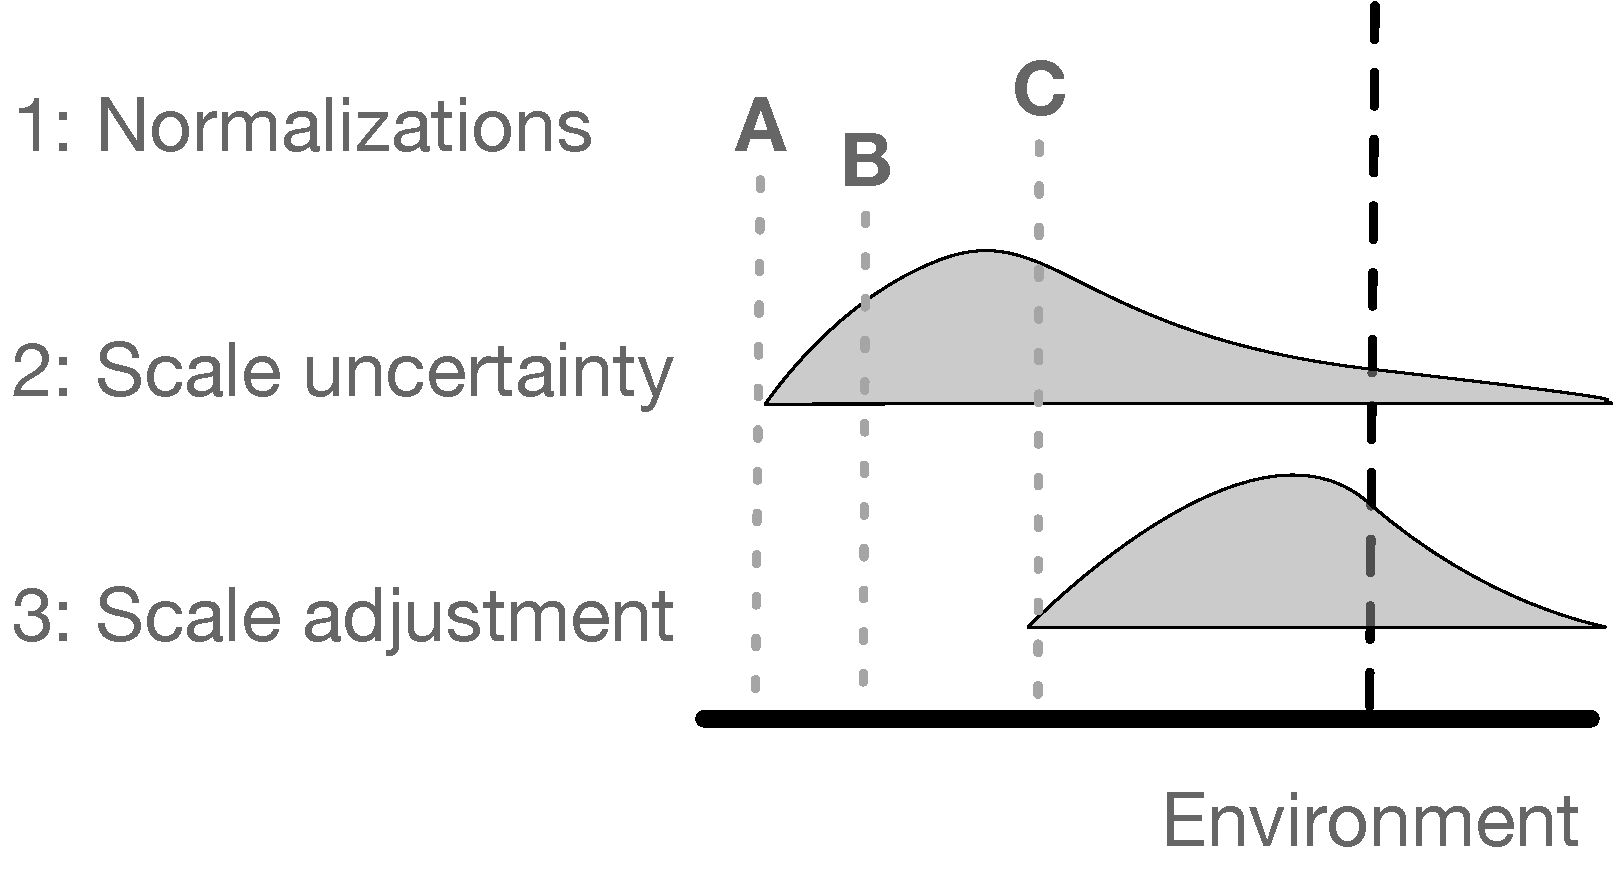
\includegraphics[width=0.6\linewidth]{./go3_files/figure-latex/scale-explained} 
%DIFDELCMD < 

%DIFDELCMD < }
%DIFDELCMD < 

%DIFDELCMD < %%%
%DIFDELCMD < \caption{%
{%DIFAUXCMD
\DIFdelFL{Mismatches between estimated scale and true scale lead to poor estimation of high throughput sequencing data. All normalizations used for differential abundance analysis make some strict assumption about the scale of the environment as shown in line 1. In this example all normalizations produce a biased estimate of the environmental scale, but estimate C is the closest to the truth.  Adding uncertainty to normalization C as represented by the distribution in the line 2 leads to less bias and now includes the actual environmental scale in the assumption. As shown in line 3 in some cases it may be useful to adjust the centre of the scale uncertainty estimate if the initial normalizations give very poor estimates of the underlying environment.}}%DIFAUXCMD
%DIFDELCMD < \label{fig:unnamed-chunk-1}
%DIFDELCMD < \end{figure}
%DIFDELCMD < 

%DIFDELCMD < %%%
\DIFdel{The original scale-naive }\DIFdelend \DIFaddbegin \DIFadd{The original naive }\DIFaddend ALDEx2 (\DIFdelbegin \DIFdel{41}\DIFdelend \DIFaddbegin \DIFadd{39}\DIFaddend ) model unwittingly made a strict
assumption about scale through the CLR normalization \DIFdelbegin \DIFdel{and we found that
the CLR was very sensitive to violations of the assumption of scale
identity between groups (15). Moreover, when the assumption of identity
was not true the CLR used by ALDEx2 }\DIFdelend \DIFaddbegin \DIFadd{(3). This
assumption was often close enough to the true value to be useful, but
was not always the a good estimate and }\DIFaddend could be outperformed by other
normalizations \DIFdelbegin \DIFdel{in simulation studies (42). As illustrated graphically in
Figure 1, }\DIFdelend \DIFaddbegin \DIFadd{(40). }\DIFaddend Nixon et al. (3) showed \DIFdelbegin \DIFdel{through simulation that introducing
uncertainty in the scale
assumptions , and in extreme cases altering the
location of the scale assumption, }\DIFdelend \DIFaddbegin \DIFadd{that better scale
assumptions }\DIFaddend resulted in more reproducible data analysis including better
control of both false positive and false negative results. We \DIFaddbegin \DIFadd{recently
}\DIFaddend modified ALDEx2 to explicitly model \DIFdelbegin \DIFdel{uncertainty in
}\DIFdelend \DIFaddbegin \DIFadd{the }\DIFaddend scale over a range of reasonable
normalization parameters, and showed significant improvements in
performance in microbiome and in-vitro selection experiments (\DIFdelbegin \DIFdel{22)and in a vaginal metatranscriptome analysis
(43)}\DIFdelend \DIFaddbegin \DIFadd{20)}\DIFaddend . Here,
we briefly review these modifications and show how \DIFdelbegin \DIFdel{adding
}\DIFdelend scale uncertainty can
greatly improve modeling in transcriptome and meta-transcriptome
datasets to provide \DIFdelbegin \DIFdel{substantially }\DIFdelend more robust and reproducible results.

\section{Implementation}\label{implementation}

Formal and expanded descriptions of the concepts that follow are given
in (3, \DIFdelbegin \DIFdel{22}\DIFdelend \DIFaddbegin \DIFadd{20}\DIFaddend ). To be concrete, we let \(\mathbf{Y}\) denote the
\emph{measured} \(D \times N\) matrix of sequence counts with elements
\(\mathbf{Y}_{dn}\) indicating the number of measured DNA molecules
mapping to feature \(d\) (e.g., a taxon, transcript or gene) in sample
\(n\). Likewise, we can denote \DIFdelbegin \DIFdel{\(\mathbf{W}_{dn}\) }\DIFdelend \DIFaddbegin \DIFadd{\(\mathbf{W}\) }\DIFaddend as the \emph{true} amount
of class \(d\) in the biological system from which sample \(n\) was
obtained. We can think of \(\mathbf{W}\) as consisting of two parts, the
scale \DIFdelbegin \DIFdel{\(\mathbf{W}^{Tot}\) }\DIFdelend \DIFaddbegin \DIFadd{\(\mathbf{W}^{\perp}\) }\DIFaddend (e.g., totals) and the composition
\DIFdelbegin \DIFdel{\(\mathbf{W}^{Comp}\) }\DIFdelend \DIFaddbegin \DIFadd{\(\mathbf{W}^{\parallel}\) }\DIFaddend (i.e., proportions). That is,
\DIFdelbegin \DIFdel{\(\mathbf{W}^{Tot}\)
}\DIFdelend \DIFaddbegin \DIFadd{\(\mathbf{W}^{\perp}\) }\DIFaddend is a \(N\)-vector with elements
\DIFdelbegin \DIFdel{\(\mathbf{W}^{Tot}_{n}=\sum_{d}\mathbf{W}_{dn}\) while
\(\mathbf{W}^{Comp}\) }\DIFdelend \DIFaddbegin \DIFadd{\(\mathbf{W}^{\perp}_{n}=\sum_{d}\mathbf{W}_{dn}\) while
\(\mathbf{W}^{\parallel}\) }\DIFaddend is a \(D \times N\) matrix with elements
\DIFdelbegin \DIFdel{\(\mathbf{W}^{Comp}_{dn}=\mathbf{W}_{dn}/\mathbf{W}^{Tot}_{n}\)}\DIFdelend \DIFaddbegin \DIFadd{\(\mathbf{W}^{\parallel}_{dn}=\mathbf{W}_{dn}/\mathbf{W}^{\perp}_{n}\)}\DIFaddend .
Note that with these definitions \(\mathbf{W}\) can be written as the
element-wise combination of scale and composition:
\DIFdelbegin \DIFdel{\(\mathbf{W}_{dn}=\mathbf{W}^{Comp}_{dn}\mathbf{W}^{Tot}_{n}\)}\DIFdelend \DIFaddbegin \DIFadd{\(\mathbf{W}_{dn}=\mathbf{W}^{\parallel}_{dn}\mathbf{W}^{\perp}_{n}\)}\DIFaddend ,
or as the logarithm
\DIFdelbegin \DIFdel{\(\log \mathbf{W}_{dn}= \log \mathbf{W}^{Comp}_{dn} + \log \mathbf{W}^{Tot}_{n}\)}\DIFdelend \DIFaddbegin \DIFadd{\(\log \mathbf{W}_{dn}= \log \mathbf{W}^{\parallel}_{dn} + \log
\mathbf{W}^{\perp}_{n}\)}\DIFaddend .

Many of the normalizations \DIFdelbegin \DIFdel{used in }\DIFdelend \DIFaddbegin \DIFadd{in widespread use in }\DIFaddend tools such as DESeq2
(\DIFdelbegin \DIFdel{44}\DIFdelend \DIFaddbegin \DIFadd{41}\DIFaddend ), edgeR (\DIFdelbegin \DIFdel{36}\DIFdelend \DIFaddbegin \DIFadd{35}\DIFaddend ), metagenomeSeq (\DIFdelbegin \DIFdel{45}\DIFdelend \DIFaddbegin \DIFadd{42}\DIFaddend ) ALDEx2 (\DIFdelbegin \DIFdel{46}\DIFdelend \DIFaddbegin \DIFadd{43}\DIFaddend ) can be stated as ratios
of the form \(\hat{{\mathbf{W}}}_{dn}
\approx \mathbf{Y}_{dn}/f(\mathbf{Y})\), where the denominator is
determined by some function of the observation. We use the
\DIFdelbegin \DIFdel{hat notation }\DIFdelend \DIFaddbegin \DIFadd{\(\hat{{\mathbf{W}}}\) }\DIFaddend (\(\ \hat{}\
\)) \DIFaddbegin \DIFadd{notation }\DIFaddend to indicate that the output is an estimate of the true
value. The technical variation in sequencing depth
\DIFdelbegin \DIFdel{,
which is often called ``library size'' has no relationship with the
actual number of molecules in the sampled environment (1) . In other
words (\(\mathbf{Y}^{Tot}_{n}=\sum_{d}\mathbf{Y}_{dn}\)) the }\DIFdelend \DIFaddbegin \DIFadd{(\(\mathbf{Y}^{\perp}_{n}=\sum_{d}\mathbf{Y}_{dn}\)) implies that
}\DIFaddend observed data \(\mathbf{Y}\) provides us with information about the
system composition \DIFdelbegin \DIFdel{\(\mathbf{W}^{Comp}\) }\DIFdelend \DIFaddbegin \DIFadd{\(\mathbf{W}^{\parallel}\) }\DIFaddend but little to no
information in the system scale \DIFdelbegin \DIFdel{\(\mathbf{W}^{Tot}\) }\DIFdelend \DIFaddbegin \DIFadd{\(\mathbf{W}^{\perp}\) }\DIFaddend (Lovell et
al.~2011).

\subsection{Adding Scale Uncertainty in
ALDEx2}\label{adding-scale-uncertainty-in-aldex2}

The ALDEx2 R package (\DIFdelbegin \DIFdel{41, 46}\DIFdelend \DIFaddbegin \DIFadd{39, 43}\DIFaddend ) is a general purpose toolbox to model the
uncertainty of HTS data and to use that model to estimate the \DIFdelbegin \DIFdel{significance of the }\DIFdelend underlying
LFC (log-fold change) \DIFaddbegin \DIFadd{significance}\DIFaddend . At a high-level, ALDEx2 has three
connected components to estimate the uncertainty inherent in HTS
datasets. First, the tool accounts for the uncertainty of the sequencing
counts using Dirichlet multinomial sampling to build a probabilistic
model of the data; i.e.,
\DIFdelbegin \DIFdel{\(\mathbf{\hat{W}}^{Comp} \approx \mathrm{Dir}(\mathbf{Y})\)}\DIFdelend \DIFaddbegin \DIFadd{\(\mathbf{\hat{W}}^{\parallel} \approx \mathrm{Dir}(\mathbf{Y})\)}\DIFaddend .
Secondly, ALDEx2 uses the centred log-ratio transformation to scale the
data (\DIFdelbegin \DIFdel{41). It was this step that was modified }\DIFdelend \DIFaddbegin \DIFadd{39). However, this step was modified recently }\DIFaddend to account for scale
uncertainty and misspecification (\DIFdelbegin \DIFdel{22) }\DIFdelend \DIFaddbegin \DIFadd{20) via a scale model, }\DIFaddend explained with
more details in (3, \DIFdelbegin \DIFdel{22}\DIFdelend \DIFaddbegin \DIFadd{20}\DIFaddend ) and summarized in the next paragraph. Finally, a
standard null-hypothesis test and a non-parametric estimate of mean
standardized difference are used to report on the finite sample
variation. These sources of uncertainty and variation are combined via
reporting the expected values from a Monte-Carlo simulation framework.
For simplicity, we use the term `difference' to refer to the absolute
difference between groups, and `dispersion' to refer to the
within-condition difference or pooled variance as defined in (\DIFdelbegin \DIFdel{41}\DIFdelend \DIFaddbegin \DIFadd{39}\DIFaddend ). These
are calculated on a \(\log_2\) scale. For more details on ALDEx2 see (3,
\DIFdelbegin \DIFdel{22, 41, 46}\DIFdelend \DIFaddbegin \DIFadd{20, 39, 43}\DIFaddend ).

Scale models \DIFdelbegin \DIFdel{were }\DIFdelend \DIFaddbegin \DIFadd{can be }\DIFaddend incorporated into ALDEx2, turning the ALDEx2 model
into a specialized type of statistical model which Nixon et al. (3) term
a \textit{Scale Simulation Random   Variable} (SSRV). To do this, Nixon
et al. (3) generalized the concept of normalizations by introducing the
concept of a \textit{scale model} to account for potential error in the
centred log-ratio normalization step. They did this by including a model
for \DIFdelbegin \DIFdel{\(\mathbf{\hat{W}}^{Tot}_{n}\)}\DIFdelend \DIFaddbegin \DIFadd{\(\mathbf{\hat{W}}^{\perp}_{n}\)}\DIFaddend . The CLR normalization used by
ALDEx2 makes the assumption \DIFdelbegin \DIFdel{\(\mathbf{\hat{W}}^{Tot}_{n}=1/G_{n}\)}\DIFdelend \DIFaddbegin \DIFadd{\(\mathbf{\hat{W}}^{\perp}_{n}=1/G_{n}\)}\DIFaddend ,
where \(G_n\) is the geometric mean of \DIFdelbegin \DIFdel{the counts (or the corresponding
proportions)of each part in }\DIFdelend sample n, which while being a
random variable, is essentially constant across each Monte-Carlo
replicate, but that differs between samples. With this modification,
ALDEx2 can be generalized by considering probability models for the
scale \DIFdelbegin \DIFdel{\(\mathbf{\hat{W}}^{Tot}_{n}\) }\DIFdelend \DIFaddbegin \DIFadd{\(\mathbf{\hat{W}}^{\perp}_{n}\) }\DIFaddend that have mean \(1/G_{n}\). For
example, the following scale model generalizes the CLR:

\[\log \mathbf{\hat{W}}\DIFdelbegin \DIFdel{^{Tot}}\DIFdelend \DIFaddbegin \DIFadd{^{\perp}}\DIFaddend _{n} = -\log G_{n} + \Lambda x_{n} \qquad \Lambda
\sim N(\mu, \gamma^{2})\DIFdelbegin \DIFdel{.}\DIFdelend \]\DIFaddbegin \DIFadd{.
}\DIFaddend 

This formulation is quite flexible (3, \DIFdelbegin \DIFdel{22}\DIFdelend \DIFaddbegin \DIFadd{20}\DIFaddend ). In the simple or `default'
configuration, \(\mu = 0\) and \(\gamma\) is a tunable parameter drawn
from a log-Normal distribution(3). Adding scale uncertainty with the
\(\gamma\) paramenter \DIFdelbegin \DIFdel{(as shown in Figure 1:1) }\DIFdelend controls only the degree of uncertainty of the CLR
assumption for the \(x_{n}\) binary condition indicator (e.g.,
\(x_{n}=1\) denotes case and \(x_{n}=0\) denotes control). In the
advanced or `informed' configuration, \(\mu\) takes different values for
each group and controls the location of the LFC assumption\DIFdelbegin \DIFdel{(as shown in Figure 1:2)}\DIFdelend ; combining
\(\mu\) with a \(\gamma\) estimate allows for uncertainty in both the
location and the scale. \DIFdelbegin \DIFdel{In
the manuscript where the idea of scale was original derived, Nixon et
al. (3) conducted extensive simulations showing that }\DIFdelend \DIFaddbegin \DIFadd{An example of }\DIFaddend both the default and informed
approaches \DIFdelbegin \DIFdel{exhibit }\DIFdelend \DIFaddbegin \DIFadd{is given for a microbiome dataset in (20) showing }\DIFaddend increased
sensitivity and specificity\DIFdelbegin \DIFdel{(22). In this report }\DIFdelend \DIFaddbegin \DIFadd{. Here }\DIFaddend we show that these approaches also
work well \DIFdelbegin \DIFdel{to
control the FDR }\DIFdelend in transcriptome and metatranscriptome datasets. \DIFdelbegin \DIFdel{We also
provide some additional insights into how this is achieved. }\DIFdelend These
modifications are instantiated in ALDEx2 which is the first software
package designed for SSRV-based inference.

\section{Results}\label{results}

\subsection{Adding scale uncertainty replaces the need for dual
significance
cutoffs.}\label{adding-scale-uncertainty-replaces-the-need-for-dual-significance-cutoffs.}

Gierliński et al. (\DIFdelbegin \DIFdel{47}\DIFdelend \DIFaddbegin \DIFadd{44}\DIFaddend ) generated a highly replicated yeast transcriptome
dataset to compare gene expression between a wild-type strain and a snf2
gene knockout, \(\Delta\)snf2. This dataset \DIFdelbegin \DIFdel{of 86 samples (44 and 42 per
group) is an example of technical growth replicate experiments common in
the literature. The dataset }\DIFdelend was used to test several
RNA-seq tools for their power to detect the set of differentially
abundant transcripts identified in the full dataset when the data was
subset (\DIFdelbegin \DIFdel{9}\DIFdelend \DIFaddbegin \DIFadd{14}\DIFaddend ). In this \DIFdelbegin \DIFdel{original }\DIFdelend study each tool had its own `gold standard' set of
transcripts with different tools identifying between between 65\% to
\textgreater80\% of all transcripts as being significantly different.
Since the majority of transcripts were significantly different, the
authors suggested that it was more appropriate to apply a dual cutoff
composed of both a Benjamini-Hochberg (\DIFdelbegin \DIFdel{48}\DIFdelend \DIFaddbegin \DIFadd{45}\DIFaddend ) corrected p-value (q-value)
plus a difference cutoff to limit the number of identified transcripts
to a much smaller fraction of the total. \DIFdelbegin \DIFdel{In other datasets, }\DIFdelend Nixon et al, (\DIFdelbegin \DIFdel{22}\DIFdelend \DIFaddbegin \DIFadd{20}\DIFaddend ) showed that
adding even a small amount of scale uncertainty with ALDEx2 dramatically
reduced the number of significant transcripts identified, removing the
need for the dual cutoff approach in this dataset and others. \DIFaddbegin \DIFadd{Below we
include an intuitive explanation of why and how incorporating scale
uncertainty achieved this outcome using a setting of \(\gamma=0.5\). The
approach is in line with the recommendations of (20) and gives results
comparable to those proposed in (14).
}\DIFaddend 

\DIFdelbegin %DIFDELCMD < \begin{figure}
%DIFDELCMD < 

%DIFDELCMD < {\centering 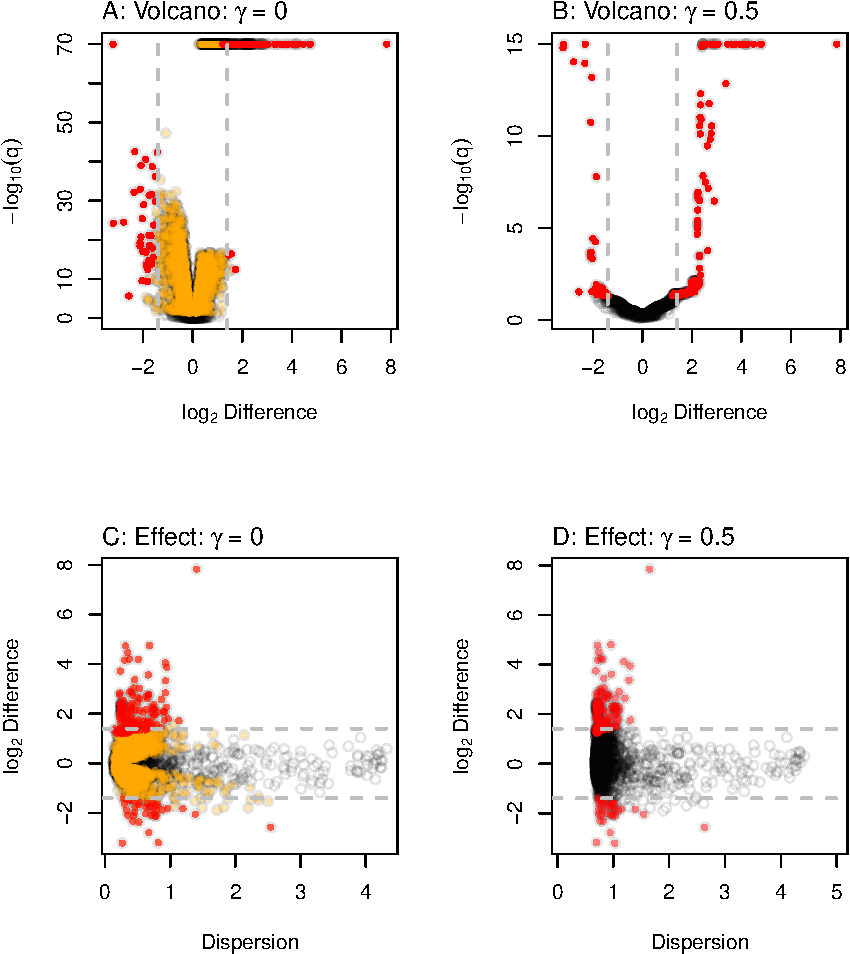
\includegraphics[width=0.8\linewidth]{go3_files/figure-latex/yst-plot-1} 
%DIFDELCMD < 

%DIFDELCMD < }
%DIFDELCMD < 

%DIFDELCMD < %%%
%DIFDELCMD < \caption{%
{%DIFAUXCMD
\DIFdelFL{Volcano and effect plots for unscaled and scaled transcriptome analysis. ALDEx2 was used to conduct a differential expression (DE) analysis on the yeast transcriptome dataset. The results were plotted to show the relationship between difference and dispersion using effect plots or difference and the q-values using volcano plots. Panels A,C are for the naive analyses, and Panels B,D are for the  default analyses that include scale uncertainty. Each point represents the values for one transcript, with the color indicating if that transcript was significant in the both analyses (red) or in the naive analysis only (orange). Points in grey are not statistically signficantly different under any condition. The horizontal dashed lines represent a \(\log_2\)difference of \(\pm 1.4\).}}%DIFAUXCMD
%DIFDELCMD < \label{fig:yst-plot}
%DIFDELCMD < \end{figure}
%DIFDELCMD < 

%DIFDELCMD < %%%
\DIFdelend We start with the assumption that not all statistically significant
differences are biologically relevant (\DIFdelbegin \DIFdel{49}\DIFdelend \DIFaddbegin \DIFadd{46}\DIFaddend ), and that \DIFdelbegin \DIFdel{a result where the
majority of transcripts are significant }\DIFdelend \DIFaddbegin \DIFadd{such a large number
of significantly different transcripts }\DIFaddend breaks the necessary assumption
for DA/DE expression that most parts be invariant (\DIFdelbegin \DIFdel{31). Transcriptomic
analysis }\DIFdelend \DIFaddbegin \DIFadd{30). As noted,
transcriptomics }\DIFaddend commonly uses a dual cutoff approach \DIFaddbegin \DIFadd{that is }\DIFaddend graphically
exemplified by volcano plots (\DIFdelbegin \DIFdel{9, 11}\DIFdelend \DIFaddbegin \DIFadd{14, 16}\DIFaddend ). Using either DESeq2 or ALDEx2, a
majority of transcripts are statistically significantly different
between groups with a q-value cutoff of \(\le 0.05\); i.e.~4636 (79\%,
DESeq2) or 4172 (71\%, ALDEx2) of the 5891 transcripts. These values are
in line with those observed by (\DIFdelbegin \DIFdel{9}\DIFdelend \DIFaddbegin \DIFadd{14}\DIFaddend ). Such large numbers of statistically
significant transcripts seems biologically unrealistic. That 118
transcripts are identified by ALDEx2 and not DESeq2, while DESeq2
identifies 582 transcripts that ALDEx2 does not, suggests that the
choice of normalization plays a role in which results are returned as
significant and that some, if not the majority, are driven by technical
differences in the analysis (\DIFdelbegin \DIFdel{8, 31)or are false positives}\DIFdelend \DIFaddbegin \DIFadd{13, 30)}\DIFaddend .

\DIFaddbegin \begin{figure}
\centering
\pandocbounded{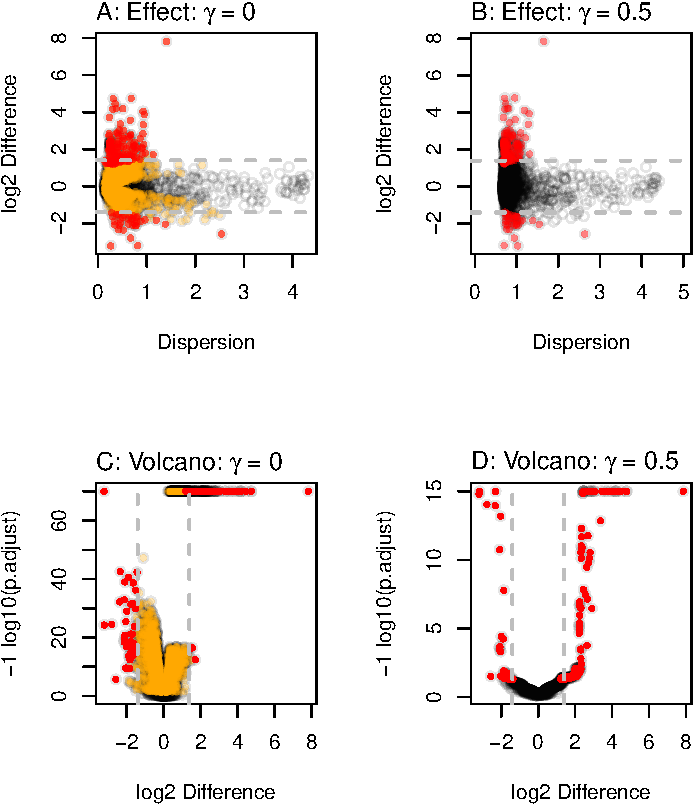
\includegraphics[keepaspectratio]{go3_files/figure-latex/plot1-1.pdf}}
\caption{\DIFaddFL{Volcano and effect plots for unscaled and scaled transcriptome
analysis. ALDEx2 was used to conduct a differential expression (DE)
analysis on the yeast transcriptome dataset. The results were plotted to
show the relationship between difference and dispersion using effect
plots or difference and the q-values using volcano plots. Panels A,C are
for the naive analyses, and Panels B,D are for the default analyses that
include scale uncertainty. Each point represents the values for one
transcript, with the color indicating if that transcript was significant
in the both analyses (red) or in the naive analysis only (orange).
Points in grey are not statistically signficantly different under any
condition. The horizontal dashed lines represent a \(\log_2\)difference
of \(\pm 1.4\).}}
\end{figure}

\DIFaddend The Volcano plots in Figure \DIFdelbegin \DIFdel{2 }\DIFdelend \DIFaddbegin \DIFadd{1 }\DIFaddend A and B show that adding scale uncertainty
increases the minimum q-value and increases the concordance between the
q-value and the difference between groups (compare panels A and B). The
effect plots (\DIFdelbegin \DIFdel{50}\DIFdelend \DIFaddbegin \DIFadd{47}\DIFaddend ) in Figure \DIFdelbegin \DIFdel{2C }\DIFdelend \DIFaddbegin \DIFadd{1C }\DIFaddend shows that the majority of significant
transcripts (red, orange) have negligible differences between groups and
very low dispersion. We suggest that this low dispersion is driven by
the experimental design which is actually a technical wet lab
replication rather than a true biological replication design (\DIFdelbegin \DIFdel{47}\DIFdelend \DIFaddbegin \DIFadd{44}\DIFaddend ). Scale
uncertainty can be incorporated using the \texttt{gamma} parameter that
controls the amount of noise added to the CLR mean assumption when we
call either \texttt{aldex()}, or \texttt{aldex.clr()}. Figure \DIFdelbegin \DIFdel{2 }\DIFdelend \DIFaddbegin \DIFadd{1 }\DIFaddend B,D
shows that setting \(\gamma=0.5\) \DIFdelbegin \DIFdel{now }\DIFdelend results in 205 which is far fewer
\DIFdelbegin \DIFdel{statistically }\DIFdelend significant transcripts than in the naive analysis and we observe that
the minimum dispersion increases from 0.12 (\(\gamma = 0\) ) to 0.67
(\(\gamma=0.5\)).

\DIFaddbegin \begin{figure}
\centering
\pandocbounded{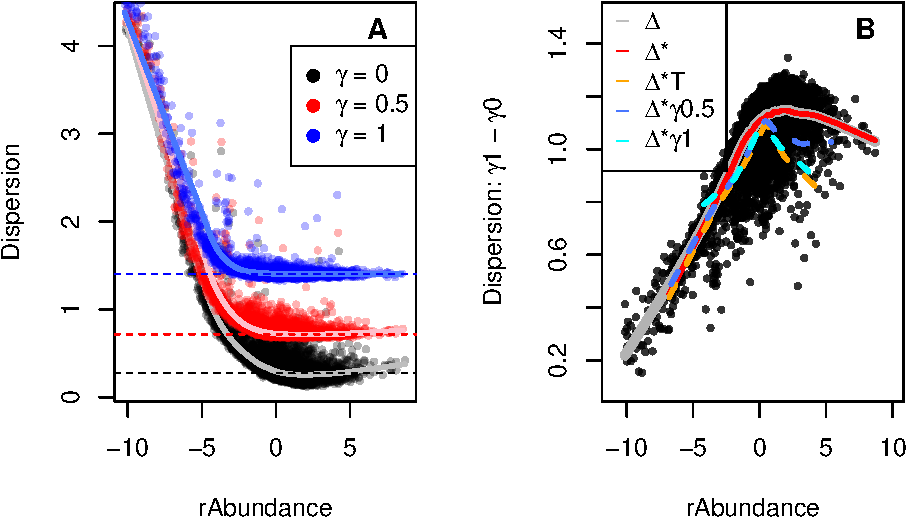
\includegraphics[keepaspectratio]{go3_files/figure-latex/disp-1.pdf}}
\caption{\DIFaddFL{Adding scale uncertainty changes the dispersion distribution.
Panel A shows a plot of the expected value for relative abundance vs the
expected value for the pooled dispersion as output by
}\texttt{\DIFaddFL{aldex.effect}}\DIFaddFL{. The dashed horizontal lines show the median value
for the features with a rAbundance between -0.5 and 0.5, and the light
colored lines are lowess lines of fit through the center of mass of the
data. Panel B plots the dispersion difference between \(\gamma = 1\) and
\(\gamma = 0\); note the non-linear relationship that highlights the
rotation that is evident in Panel A. The colored lines indicate the
lowess line of fit through the centre of mass of the plot for the
various populations of points. The grey line is the total population and
shows the difference \(\Delta\), the red line is the population of
significant transcripts (*) with \(\gamma = 0\), the orange line is the
population of significant transcripts with a difference threshold (T) of
about \(\pm 2^{1.4}\)-fold change, the blue line is the population of
significant transcripts with \(\gamma = 0.5\), and the cyan line is the
significant population with \(\gamma = 1\). \(\Delta\): Difference, *:
significant, T: thresholded.}}
\end{figure}

\DIFaddend It is common practice to use a dual-cutoff by choosing transcripts based
on a thresholds for both q-values and fold-changes (\DIFdelbegin \DIFdel{9), and these were
first proposed for microarray experiments through volcano plots (11}\DIFdelend \DIFaddbegin \DIFadd{14, 16}\DIFaddend ). Note that
there is considerable variation in recommended cutoff values(\DIFdelbegin \DIFdel{9), and that this controversy has persisted ever since fold-change was
suggested (51). Unfortunately,
universal cutoff fold-change values
cannot be identified in part because different tools have intrinsically
different variance in their log\_2-fold change ranges (52). This has led
to the widespread practice of applying a post-hoc fold-change cutoff to
reduce the number of positive identifications to a manageable proportion
of the whole dataset. Here, we applied the }\DIFdelend \DIFaddbegin \DIFadd{14). Here,
applying a }\DIFaddend dual-cutoff \DIFdelbegin \DIFdel{method using a fold-change }\DIFdelend \DIFaddbegin \DIFadd{using a heuristic }\DIFaddend of at least a \(2^{1.4}\) fold
change \DIFdelbegin \DIFdel{that }\DIFdelend reduces the number of significant outputs to 193 for DESeq2 and
to 186 for ALDEx2. This cutoff was chosen for convenience and is \DIFdelbegin \DIFdel{mid-way between the high
and low fold-change }\DIFdelend \DIFaddbegin \DIFadd{in-line
with the }\DIFaddend recommendations of (\DIFdelbegin \DIFdel{9) . These limits are }\DIFdelend \DIFaddbegin \DIFadd{14) with the fold change limits }\DIFaddend shown by
the dashed grey lines in Figure \DIFdelbegin \DIFdel{2 and we can see that a }\DIFdelend \DIFaddbegin \DIFadd{1. The }\DIFaddend \(2^{1.4}\) fold change \DIFdelbegin \DIFdel{\((\sim 2.6\) fold) }\DIFdelend cutoff
identifies a similar number of transcripts as does ALDEx2 using
\(\gamma = 0.5\) which identifies \DIFdelbegin \DIFdel{205
transcripts.
}%DIFDELCMD < 

%DIFDELCMD < %%%
\DIFdelend \DIFaddbegin \DIFadd{205. }\DIFaddend Supplementary Figures 1 \DIFdelbegin \DIFdel{shows an example of }\DIFdelend \DIFaddbegin \DIFadd{and 2
shows how to use }\DIFaddend the \texttt{aldex.senAnalysis()} function to identify
those transcripts that are very sensitive to scale uncertainty\DIFdelbegin \DIFdel{in this dataset. Here }\DIFdelend \DIFaddbegin \DIFadd{. In this
supplementary figure }\DIFaddend we see that \DIFaddbegin \DIFadd{even }\DIFaddend adding a very small amount of
scale \(\gamma = 0.1\) reduces the number of significant transcripts by
more than half\DIFdelbegin \DIFdel{in the yeast
dataset}\DIFdelend . This allows \DIFdelbegin \DIFdel{the analyst }\DIFdelend \DIFaddbegin \DIFadd{us }\DIFaddend to ignore those low-dispersion
transcripts that were significant only because of an absence of scale
uncertainty. \DIFdelbegin %DIFDELCMD < 

%DIFDELCMD < %%%
\DIFdel{We next examined how adding scale would alter the analysis in a real
dataset to which synthetically generated true positive counts had been
added. We show results from the anti-PD-1 therapy RNA-seq dataset (53)which examined changes in gene expression when cells were exposed or not
to a cell-cycle checkpoint inhibitor.
This dataset was used by Li et al.
(8) as an example of the dangers of relying on tools with high false
positive error rates when analyzing clinical or clinically-related
transcriptome samples. Indeed, in the benchmarking analysis done by this
group, they found that parameter based methods such as DESeq2 and edgeR
that on reported p-value }\DIFdelend \DIFaddbegin \DIFadd{In practice, we suggest that a }\texttt{\DIFadd{gamma}} \DIFadd{parameter
between 0.5 }\DIFaddend and \DIFdelbegin \DIFdel{fold-change cutoffs often led to
conclusions in the original dataset that were indistinguishable from
permutations of the dataset. In other words, that the analysis of
transcriptome datasets from patient-derived samples often exhibited many
false-positive identifications.
}\DIFdelend \DIFaddbegin \DIFadd{1 is realistic for most experimental designs (20).
}\DIFaddend 

\DIFdelbegin %DIFDELCMD < \begin{figure}
%DIFDELCMD < %%%
\DIFdelendFL \DIFaddbeginFL \DIFaddFL{The effect on dispersion with increasing amounts of scale uncertainty
are shown in Figure 2A, where we can see that the dispersion increases
as uncertainty is added. Note that the dispersion in the unscaled
analysis in Figure 2A reaches a minimum near the mid-point of the
distribution, and also does so when the analysis is conducted with
DESeq2 (Supplementary Figure 3). This shows more clearly that dispersion
of many transcripts is almost negligible in the absence of scale
uncertainty. This plot makes the counter-intuitive suggestion that the
variance in expression of the majority of genes with moderate expression
is more predictable than highly-expressed genes or of housekeeping genes
(48). This is at odds with the known biology of cells where single cell
counting of highly-expressed transcripts shows that they have little
intrinsic variation (23, 49).
}\DIFaddendFL 

\DIFdelbeginFL %DIFDELCMD < {\centering 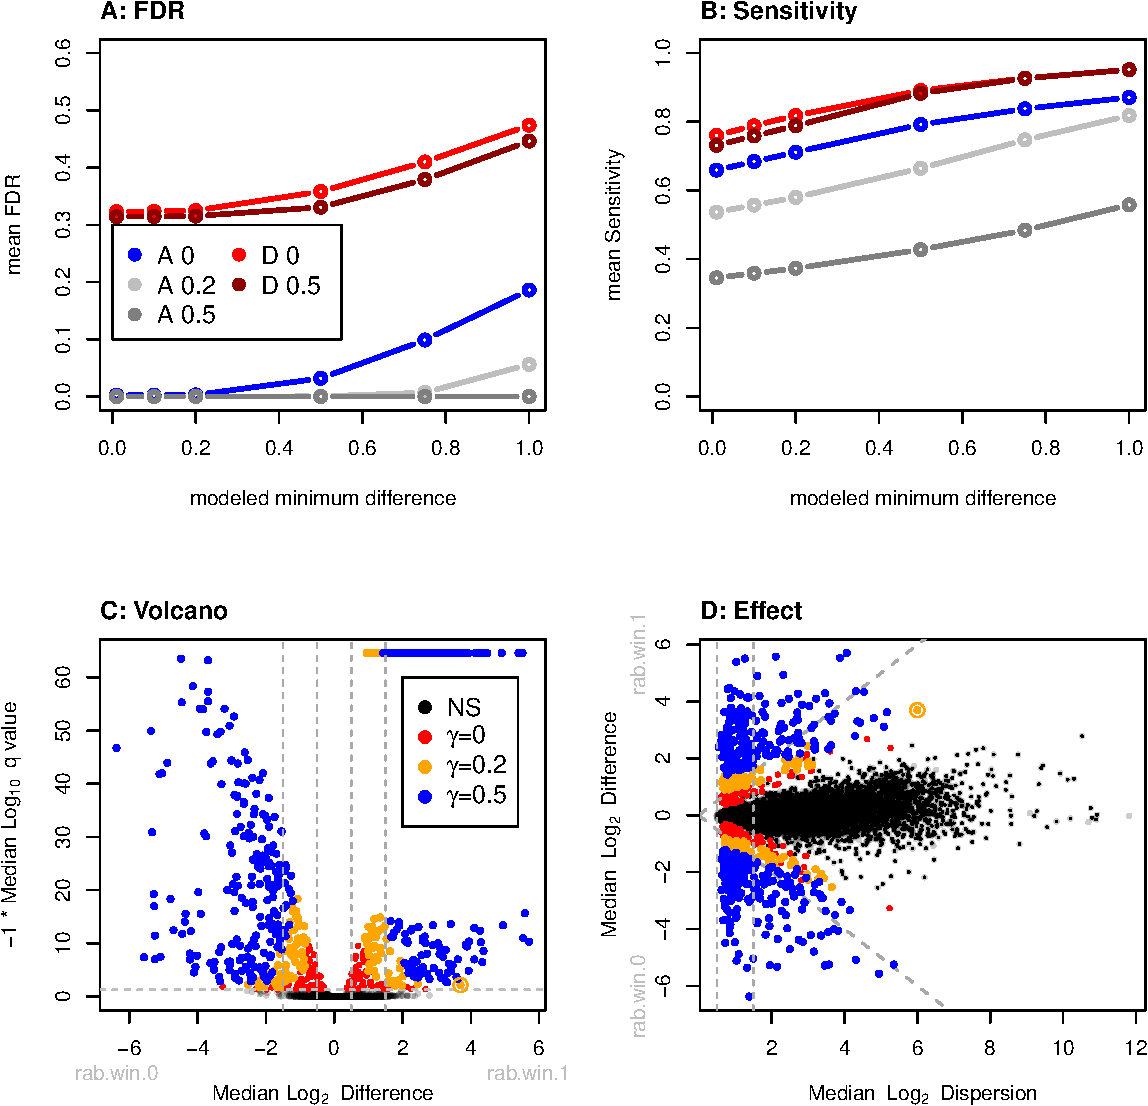
\includegraphics[width=0.8\linewidth]{go3_files/figure-latex/immuno-1} 
%DIFDELCMD < 

%DIFDELCMD < }
%DIFDELCMD < 

%DIFDELCMD < %%%
%DIFDELCMD < \caption{%
{%DIFAUXCMD
\DIFdelFL{Results of modeling true positive (TP) differences in the PD-1 dataset. For this the data were shuffled and  5\% of the transcripts were modeled to have TP differences between groups where the differences were drawn from a Normal distribution with a mean difference of 0 and a sd of 2. Panel A shows the mean FDR of 10 instances for scale-naive ALDEx2 (A 0), and ALDEx2 with \(\gamma=0.2\) (A 0.2) or \(\gamma=0.2\) (A 0.5), and where significant features were identified by  DESeq2 without (D 0), or with (D 0.5) a 0.5-fold change difference. The x-axis shows how the FDR changes for each tool as a function of the estimated modeled difference between groups. Panel B shows the mean sensitivity (TP found /all TP). Panels C and D show volcano and effect plots for the ALDEx2 output with the transcripts identified as significant at each scale setting as colored points, and non-significant transcripts in black.}}%DIFAUXCMD
%DIFDELCMD < \label{fig:immuno}
%DIFDELCMD < \end{figure}
%DIFDELCMD < 

%DIFDELCMD < %%%
\DIFdel{Figure 3 shows the results of ten permutations of this dataset while
simulating 5\% of the
transcripts to be true positives where the
difference from no change was derived from a Normal distribution(54).
This simulation was conducted with
}\DIFdelend \DIFaddbegin \DIFadd{Adding scale uncertainty by setting \(\gamma=0.5\) , or
\(\gamma = 1.0\), increases the minimum dispersion as shown in Figure 2A
by the red and blue data points, and by the colored lines of fit through
the centre of mass of }\DIFaddend the \DIFdelbegin \texttt{\DIFdel{seqgendiff}} %DIFAUXCMD
\DIFdel{R package
(54)to both permute the dataset and to add true positive features. We
did ten permutations and kept track of }\DIFdelend \DIFaddbegin \DIFadd{data. Less obvious is that }\DIFaddend the \DIFdelbegin \DIFdel{number of true and false
positive identifications. Figure 3A shows the actual false discovery
rate for ALDEx2 with and without the addition of scale
uncertaintyand
for DESeq2 with or without a fold-change cutoff of \(2^{0.5}\). When the modeled difference was greater than 0, ALDEx2 exhibited a FDR of
\(\gamma = 0\): 0.002, \(\gamma = 0.2\): 0, and \(\gamma = 0.5\): 0,
while DESeq2 with no fold-change cutoff had an FDR of 0.32 and with a
0.5 fold-change cutoff an FDR of 0.31. Figure 3 also plots these results
as a function of the
minimum modelled fold change of the true positive
transcripts. First, we can see that this analysis recapitulates the
observations of Li et al (8)in that DESeq2 has very poor false positive
control at a nominal FDR of 0.05. The FDR is not controlled any better
when a fold-change cutoff is applied, and this agrees with previous work
showing that fold-change cutoffs do not materially improve FDR control
in high throughput datasets (12, 13).
}\DIFdelend \DIFaddbegin \DIFadd{additional
dispersion is not applied equally to all points. }\DIFaddend Figure \DIFdelbegin \DIFdel{3B shows that DESeq2 has
higher sensitivity than does ALDEx2, and not surprisingly this
sensitivity increases as }\DIFdelend \DIFaddbegin \DIFadd{2B shows a plot
of the difference between }\DIFaddend the \DIFdelbegin \DIFdel{difference between groups increases. For
the case where the mean difference is 0 or greater, ALDEx2 exhibited a
sensitivity of \(\gamma = 0\): 0.66, \(\gamma = 0.2\): 0.54, and \(\gamma = 0.5\): 0.35, while DESeq2 with no fold-change cutoff had a
sensitivity of 0.76 and with a 0.5 fold-change cutoff a sensitivity of
0.73. In this example, scale-naive ALDEx2 has near perfect FDR control
and reasonable sensitivity at low modeled difference between groups.
However, when the modeled difference between groups becomes large, then
the scale-naive version of ALDEx2 begins to exhibit unacceptable rates
of false positives and the false positive rate for DESeq2 also
increases. Adding in even small amounts of scale uncertainty drops the
true FDR rate to 0, but at the expense of sensitivity. The major
contributor to the increase in FDR with larger modeled differences is
that the tools are identifying as positives those transcripts that are
modeled to have differences just below the threshold. We need to
recognize that there is no such thing as a statistical free lunch; the
analyst can have high sensitivity but low confidence that any individual
transcript is truly different, or have lower sensitivity but have very
high confidence that the difference is real. In other words, the
sensitivity of a method is directly tied to how much error the
investigator is willing to tolerate. }%DIFDELCMD < 

%DIFDELCMD < %%%
\DIFdel{Examination of the volcano plot (11) and effect plot (50) in Figure 3C
and D provides some insight into why adding scale uncertainty provides
better FDR control than does the approach of using a p-value and a
fold-change cutoff. In the volcano plot
, adding scale uncertainty
differentially excludes transcripts with a combination of marginal
p-values and low difference between groups, and }\DIFdelend \DIFaddbegin \DIFadd{\(\gamma= 0\) and \(\gamma= 1\) data and
here we can see that scale uncertainty is preferentially increasing the
dispersion of the mid-expressed transcripts }\DIFaddend that \DIFdelbegin \DIFdel{this becomes more
pronounced with a larger scale value. This effect is also seen in Figure
2 but is more nuanced. In contrast, the
fold-change cutoff does not
incorporate the magnitude of the p-value and so transcripts with large
differences, but marginal p-values are retained. The effect plot in
Figure 3D shows that the transcripts with marginal p values and large
differences that are excluded when scale uncertainty is added are those
that have a large dispersion.
}%DIFDELCMD < 

%DIFDELCMD < %%%
\DIFdel{As a concrete example consider the point that is circled in panels C and
D with a marginal p-value, with a difference between of nearly 4 and a
dispersion of greater than 6. This transcript is no longer significant
when \(\gamma = 0.2\), but would require a very large fold-change cutoff
to be excluded by the standard approach. In addition, transcripts with
very small dispersion and very small differences are also excluded when
scale uncertainty is added. Thus, the addition of scale uncertainty
achieves the desired outcome of lowering the FDR for those }\DIFdelend \DIFaddbegin \DIFadd{formerly had negligible
dispersion; examine the grey line of best fit (overlaid by the red line)
for the trend. Panel B also shows the trend of the expression-dispersion
relationship for }\DIFaddend transcripts that are \DIFdelbegin \DIFdel{either marginally differentially abundant, or where the
underlying dispersion--and hence the uncertainty in measurement--is very
high, or for transcripts that fit both criteria. }%DIFDELCMD < 

%DIFDELCMD < %%%
\DIFdel{Supplementary Figure 2 shows a second permuted dataset with the addition
of modeled differences between groups. Here we used another real dataset
with over 200 biological replicates of BRCA1 tumor and control tissue
samples from Li et al. (8). This Supplementary Figure shows that the FDR
control of DESeq2 is somewhat better than in the PD-1 dataset, although
still much greater than the the anticipated 5\%. Further, a fold-change
cutoff reduces the FDR of DESeq2 from about 30\% to just over 20\% with
a power of over 80\%. However, we can see that scale-naive ALDEx2
performs substantially better with a negligible FDR and comparable
power. Adding scale
uncertaintyagain improves FDR even for those
transcripts modeled to have larger differences and }\DIFdelend \DIFaddbegin \DIFadd{classed as statistically
significant. The red line shows }\DIFaddend the \DIFdelbegin \DIFdel{power is
substantially better than in the PD-1 dataset, reaching the same power
as DESeq2 or scale-naive ALDEx2 when the modeled difference is large. As
before, this is driven by removing from consideration those
transcripts with either a small difference between or a marginal p-value, or both.
}\DIFdelend \DIFaddbegin \DIFadd{trendline with no added scale
uncertainty, and this trendline exactly overlays with the grey trendline
for the bulk of transcripts. The orange trendline indicates those
transcripts that are both statistically significant and that have a
thresholded expression level of \(\pm 1.4\), and the dark blue and cyan
lines show the statistically significant trendline for \(\gamma=0.5\) ,
or \(1.0\).
}\DIFaddend 

\DIFdelbegin \DIFdel{Supplementary Figures 3 shows that effect of applying \(\gamma = 0.5\)
to this dataset results in reducing the number of positive transcripts
from being \(\sim 70\)\% of the whole dataset to less than 10\% of the
dataset and that this is largely because of a
reduction in significance
of those transcripts with low dispersion. Supplementary Figures 4 shows
a sensitivity analysis of the BRCA1 dataset showing that different scale
uncertainty amounts alter the number of significant transcripts in a
biological replicate experiment similarly to a technical replicate
experiment.
Supplementary Figures 5 and 6 delve into how }\DIFdelend \DIFaddbegin \DIFadd{Thus, taking Figures 1 and 2 together }\DIFaddend adding scale uncertainty \DIFdelbegin \DIFdel{affects the variace-abundance relationship in subtle ways,
and may help readers to understand the observations seen in Figure 3 and
supplementary Figure 2.
}%DIFDELCMD < 

%DIFDELCMD < %%%
\DIFdel{Together the results in this section show that adding scale uncertainty
}\DIFdelend has the
desirable effect of \DIFdelbegin \DIFdel{altering the }\DIFdelend \DIFaddbegin \DIFadd{changing the distribution of }\DIFaddend transcripts identified
as significantly different between groups\DIFdelbegin \DIFdel{in a way that exhibits better
control of FDR albeit with a corresponding reduction in sensitivity}\DIFdelend . Those parts that were
statistically significantly different \emph{only because of low
dispersion} \DIFdelbegin \DIFdel{or that }\emph{\DIFdel{had marginal p-values}} %DIFAUXCMD
\DIFdel{or both,
are now }\DIFdelend \DIFaddbegin \DIFadd{are }\DIFaddend preferentially excluded from statistical significance
\DIFdelbegin \DIFdel{. In
practice, we suggest that a }\texttt{\DIFdel{gamma}} %DIFAUXCMD
\DIFdel{parameter of between 0.2 and
0.5 is realistic for most experimental designs (22) regardless if the
replication is technical or biological}\DIFdelend \DIFaddbegin \DIFadd{while those parts that were significantly different because of a high
difference between groups remain}\DIFaddend .

\subsection{Housekeeping genes and functions to guide scale model
choices.}\label{housekeeping-genes-and-functions-to-guide-scale-model-choices.}

Dos Santos et al. (\DIFdelbegin \DIFdel{55}\DIFdelend \DIFaddbegin \DIFadd{50}\DIFaddend ) used a vaginal metatranscriptome dataset to
compare the gene expression in bacteria collected from healthy (H) and
bacterial vaginosis (BV) affected women. \DIFdelbegin \DIFdel{This dataset is derived from
two publicly available datasets composed of a set of 20 non-pregnant
women from London, Ontario Canada (56) and a subset of 22 non-pregnant
women collected from German women who underwent metronidazole treatment
for BV (57). Batch effects for these two groups were removed with
ComBat-seq (58) and the two datasets were merged into one, giving a
total of 16 H and 26 BV samples. In the Dos Santos paper, all results
from this initial analysis were replicated in a much larger dataset
derived from the MOMS-PI study (59)
}%DIFDELCMD < 

%DIFDELCMD < %%%
\DIFdel{In this vaginal }\DIFdelend \DIFaddbegin \DIFadd{In this }\DIFaddend environment, both the
relative abundance of species between groups and the gene expression
level within a species is different (\DIFdelbegin \DIFdel{60}\DIFdelend \DIFaddbegin \DIFadd{51}\DIFaddend ). Additionally, prior research
suggests that the total number of bacteria is about 10 times more in the
BV than in the H condition (\DIFdelbegin \DIFdel{28}\DIFdelend \DIFaddbegin \DIFadd{26}\DIFaddend ). Thus, these are extremely challenging
datasets in which to determine differential abundance as there are both
compositional and scale changes between conditions. The usual method to
analyze vaginal metratranscriptome data is to do so on an
organism-by-organism basis (\DIFdelbegin \DIFdel{57, 59, 60}\DIFdelend \DIFaddbegin \DIFadd{51--53}\DIFaddend ) because the scale confounding of the
environment is less pronounced. One attempt at system-wide analysis
returned several housekeeping functions as differentially expressed
between groups (\DIFdelbegin \DIFdel{57}\DIFdelend \DIFaddbegin \DIFadd{52}\DIFaddend ); a result likely due to a disconnect between the
assumptions of the normalization used and the actual scale of the
environment (\DIFdelbegin \DIFdel{15}\DIFdelend \DIFaddbegin \DIFadd{19}\DIFaddend ).

\DIFdelbegin %DIFDELCMD < \begin{figure}
%DIFDELCMD < \centering
%DIFDELCMD < \pandocbounded{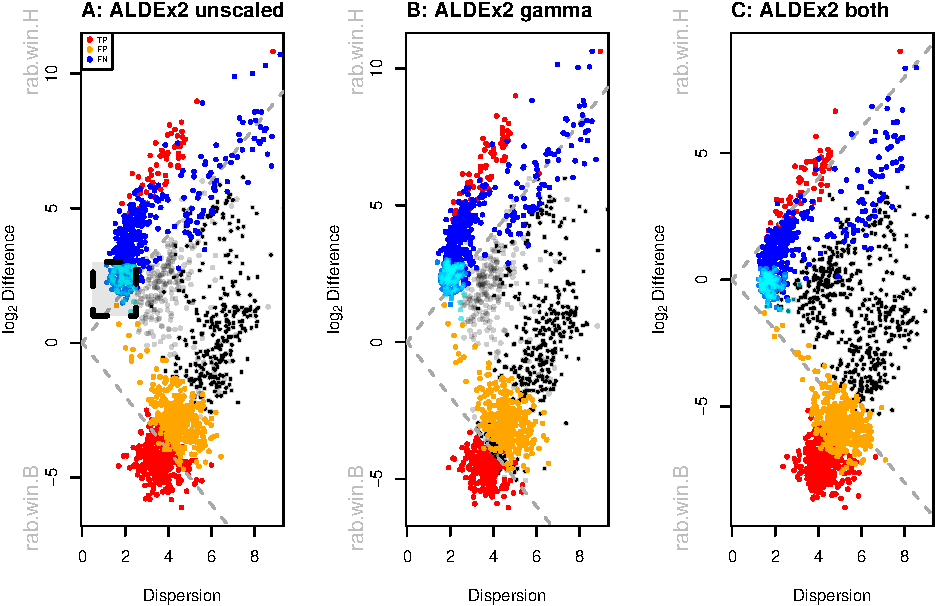
\includegraphics[keepaspectratio]{go3_files/figure-latex/meta-1.pdf}}
%DIFDELCMD < %%%
%DIFDELCMD < \caption{%
{%DIFAUXCMD
\DIFdelFL{Analysis of vaginal transcriptome data aggregated at the Kegg
Orthology (KO) functional level. Panel A shows an effect plot for the
default analysis where the functions that are elevated in the healthy
individuals have positive values and functions that are elevated in BV
have negative values. Highlighed in the box are KOs that are almost
exlusively housekeeping functions; these and are colored cyan. These
housekeeping functions should be located on the midline of no
difference. Panel B shows the same data scaled with \(\gamma = 0.5\),
which increase the minimum dispersion as before. Panel C shows the same
data scaled with \(\gamma = 0.5\) and a 0.14 fold difference in
dispersion applied to the BV samples relative to the H samples. In these
plots statistically significant (q-value \textless{} 0.01) functions in
the informed model are in red, false positive functions are in blue,
non-significant functions in black and false negative functions are in
orange.}}
%DIFAUXCMD
%DIFDELCMD < \end{figure}
%DIFDELCMD < 

%DIFDELCMD < %%%
\DIFdelend In this example, we show how to specify and interpret \DIFdelbegin \DIFdel{a user defined or
}\emph{\DIFdel{informed}} %DIFAUXCMD
\DIFdelend \DIFaddbegin \DIFadd{an informed }\DIFaddend scale
model that can explicitly account for some of these modeling
difficulties (\DIFdelbegin \DIFdel{22}\DIFdelend \DIFaddbegin \DIFadd{20}\DIFaddend ) even in a difficult \DIFdelbegin \DIFdel{to analyze }\DIFdelend dataset. An informed scale model
can control for both the mean difference of scale between groups (e.g.,
directly incorporate information on the differences in total number of
bacteria between the BV and H conditions) as well as the uncertainty of
that difference\DIFdelbegin \DIFdel{as illustrated in Figure
1:3. }\DIFdelend \DIFaddbegin \DIFadd{. }\DIFaddend To specify a user-defined scale model, we can pass a
matrix of scale values instead of an estimate of just the scale
uncertainty to \texttt{aldex.clr()}. This matrix should have the same
number of rows as the of Monte-Carlo Dirichlet samples, and the same
number of columns as the number of samples. While this matrix can be
computed from scratch by the analyst, there is an
\texttt{aldex.makeScaleModel()} function that can be used to simplify
this step in most cases. This encodes the scale model as
\(\Lambda \sim N(log_2 \mu_n,
\gamma^{2})\), where \(\mu_n\) represents the scale value for each
sample or group and \DIFdelbegin \DIFdel{\(gamma\) }\DIFdelend \DIFaddbegin \DIFadd{gamma }\DIFaddend is the uncertainty as before. The scale
estimate can be a measured value (cell count, nucleic acid input, \DIFdelbegin \DIFdel{spike-ins, }\DIFdelend etc)
or an estimate. Nixon et al. (3, \DIFdelbegin \DIFdel{22}\DIFdelend \DIFaddbegin \DIFadd{20}\DIFaddend ) showed that only the ratio of the
means are important when providing values for \(\mu_n\); i.e., the ratio
between the \(\log_2 \mu_i\) and \(\log_2 \mu_j\) values. See the
supplement to Nixon et al. (\DIFdelbegin \DIFdel{22}\DIFdelend \DIFaddbegin \DIFadd{20}\DIFaddend ) for more information.

Figure \DIFdelbegin \DIFdel{4A }\DIFdelend \DIFaddbegin \DIFadd{3A }\DIFaddend shows an effect plot of the data where reads are grouped by
homologous function regardless of the organism of origin. Each point
represents one of 3728 KEGG functions (\DIFdelbegin \DIFdel{61}\DIFdelend \DIFaddbegin \DIFadd{54}\DIFaddend ). There are many more
functions represented in the BV group (bottom) than in the healthy group
(top). This is because the \textit{Lactobacilli} that dominate a healthy
vaginal microbiome have reduced genome content relative to the anaerobic
organisms that dominate in BV, because there is a greater diversity of
organisms in BV than in H samples, and because the BV condition has
about an order of magnitude more bacteria than does the H condition.

The naive scale model appears to be reflecting the bacterial load as
observed by calculating the mean scale value for each group. Using a
negligible scale value; i.e., \(\gamma=1e-3\) exposes the naive scale
estimate for samples in the \texttt{@scaleSamps} slot from the
\texttt{aldex.clr} output. \DIFdelbegin \DIFdel{The }\DIFdelend \DIFaddbegin \DIFadd{the }\DIFaddend naive scale estimate for the
\DIFaddbegin 

\DIFaddend healthy group is 17.41 and for the BV group is 14.59 for a difference of
2.82. This is interpreted as the scale of the H group of samples being
7.06 greater than the BV group. \DIFaddbegin \DIFadd{This precise but incorrect estimate
places the location of the housekeeping genes off the midline of no
difference.
}\DIFaddend 

Applying the default scale model of \(\gamma=0.5\) increases the
dispersion slightly but does not move the housekeeping functions toward
the midline. This is as expected; the mean of the default scale model is
based on the CLR normalization so no shift in location would be expected
over the \DIFdelbegin \DIFdel{scale-naive }\DIFdelend \DIFaddbegin \DIFadd{original }\DIFaddend ALDEx2 model. Nevertheless, about 30\% of the
housekeeping functions are no longer statistically significantly
different. Note that this change is simple to conduct, has no additional
computational complexity and requires only a slight modification for the
analyst.

There are 101 functions with low dispersion that appear to be shared by
both groups (boxed area in Figure 3A, and colored in cyan). Inspection
shows that these largely correspond to core metabolic functions such as
transcription, translation, ribosomal functions, glycolysis,
replication, chaperones, etc (Supplementary file housekeeping.txt). The
transcripts of many of these are commonly used as invariant reference
sequences in wet lab experiments (\DIFdelbegin \DIFdel{62}\DIFdelend \DIFaddbegin \DIFadd{48}\DIFaddend ) and so are not be expected to
contribute to differences in ecosystem behaviour. \DIFdelbegin \DIFdel{Because we expect
housekeeping functions to be nearly invariant in their expression and to
occur in all organisms, the }\DIFdelend \DIFaddbegin \DIFadd{The }\DIFaddend average location
of these should be centred on 0 difference to represent an internal
reference set. However, \DIFdelbegin \DIFdel{with
the naive }\DIFdelend \DIFaddbegin \DIFadd{without an informed }\DIFaddend scale model, the mean of
these housekeeping functions is approximately located at \DIFaddbegin \DIFadd{+}\DIFaddend 2.3.
\DIFdelbegin \DIFdel{Thus, we }\DIFdelend \DIFaddbegin 

\begin{figure}
\centering
\pandocbounded{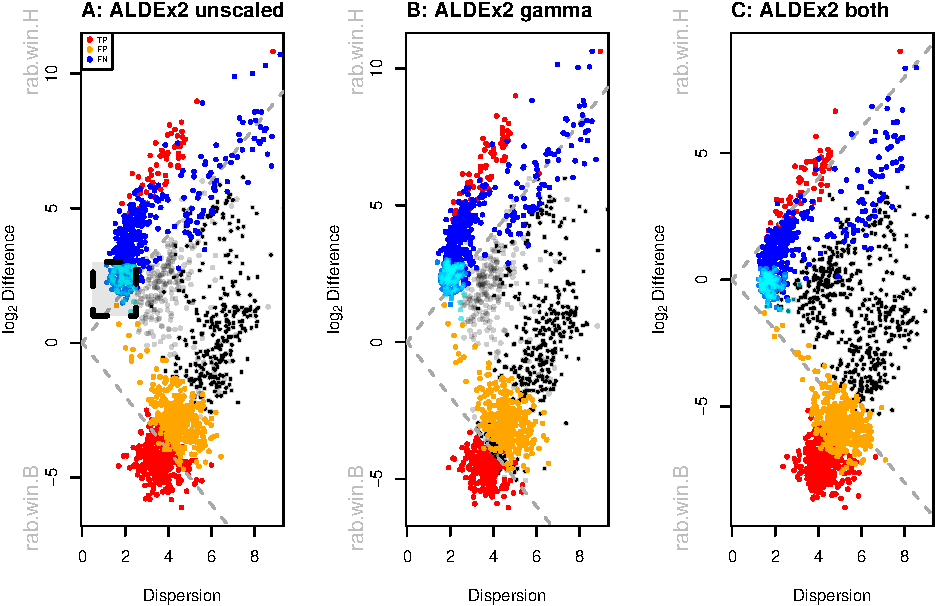
\includegraphics[keepaspectratio]{go3_files/figure-latex/meta-1.pdf}}
\caption{\DIFaddFL{Analysis of vaginal transcriptome data aggregated at the Kegg
Orthology (KO) functional level. Panel A shows an effect plot for the
default analysis where the functions that are elevated in the healthy
individuals have positive values and functions that are elevated in BV
have negative values. Highlighed in the box are KOs that are almost
exlusively housekeeping functions; these and are colored cyan. These
housekeeping functions should be located on the midline of no
difference. Panel B shows the same data scaled with \(\gamma = 0.5\),
which increase the minimum dispersion as before. Panel C shows the same
data scaled with \(\gamma = 0.5\) and a 0.14 fold difference in
dispersion applied to the BV samples relative to the H samples. In these
plots statistically significant (q-value \textless{} 0.01) functions in
the informed model are in red, false positive functions are in blue,
non-significant functions in black and false negative functions are in
orange.}}
\end{figure}

\DIFadd{We }\DIFaddend desire a scale model that approximately centres the housekeeping
functions\DIFdelbegin \DIFdel{and }\DIFdelend \DIFaddbegin \DIFadd{, because we expect housekeeping functions tp be nearly
invariant; thus }\DIFaddend an appropriate scale in this dataset for functional
analysis \DIFdelbegin \DIFdel{will place these functions
}\DIFdelend \DIFaddbegin \DIFadd{is likely }\DIFaddend closer to 0 than \DIFdelbegin \DIFdel{does }\DIFdelend the naive estimate. One way to
choose an appropriate value for \(\mu_n\) is to use the
\texttt{aldex.clr} function on only the presumed invariant functions
setting \(\gamma > 0\), and then accessing the \texttt{@scaleSamps} slot
as before. Doing so suggests that the difference in scale should be
about 14\%. A second approach would be to identify the functions used as
the denominator with the \texttt{denom="lvha"} option (\DIFdelbegin \DIFdel{15}\DIFdelend \DIFaddbegin \DIFadd{19}\DIFaddend ) for the
\texttt{aldex.clr} function, and then to use these values as before.
This approach suggests a 5\% difference in scale, and is potentially
less subject to user interpretation.

For the purposes of this example, if we assume a 14\% difference in
scale, we can set \(\mu_i = 1\) and \(\mu_j = 1.14\) using the
\texttt{makeScaleMatrix} function. This function uses a logNormal
distribution to build a scale matrix given a user-specified mean
difference between groups and uncertainty level. Applying a per-group
relative differential scale of 0.14 moves the housekeeping functions
close to the midline of no difference (Figure 3C, assuming 14\% mean
difference = -0.24, assuming a 5\% mean difference = -0.34), and
applying a gamma of 0.5 provides the same dispersion as in panel B of
Figure 3. Note that now a significant number of functions are
differentially up in BV that were formerly classed as not different
without the full scale model (orange), or when only a default scale was
applied. Inspection of the functions shows that these are largely
missing from the \emph{Lactobacillus} species and so should actually be
captured as differentially abundant in the BV group. Supplementary
Figure \DIFdelbegin \DIFdel{7 }\DIFdelend \DIFaddbegin \DIFadd{4 }\DIFaddend shows that the using either the 5\% or the 14\% scale
difference give imperceptibly different results suggesting that an
informed scale model does not have to precisely estimate the scale
difference to be useful. Nixon et al, (\DIFdelbegin \DIFdel{22}\DIFdelend \DIFaddbegin \DIFadd{20}\DIFaddend ) also found that multiple
reasonable estimates for the \(\mu_n\) part of the informed scale model
were similarly useful in microbiome data.

Thus, applying an informed scale allows us to distinguish between both
false positives (housekeeping functions in cyan, and others in blue) and
false negatives (orange functions) even in a very difficult to analyze
dataset. \DIFdelbegin \DIFdel{We used this scale model to uncover hiter-to-now unknown
differences in microbiome functional activity between the Healthy and BV
cohorts that were missed in previos analyses and that explain important
clinical differences between them (55). }\DIFdelend The remarkable improvements in biological interpretation
afforded by an informed scale model, and the transferrability of it
between sample cohorts of the same condition is outlined \DIFdelbegin \DIFdel{in dos Santos et al. (55}\DIFdelend \DIFaddbegin \DIFadd{elsewhere (50}\DIFaddend ).
We suggest that the default scale model is sufficient when the data are
approximately centred\DIFdelbegin \DIFdel{but that }\DIFdelend \DIFaddbegin \DIFadd{. However, }\DIFaddend an informed model is more appropriate
with datasets are not well centred or when the investigator has prior
information about the underlying biology.

\section{Discussion}\label{discussion}

\DIFdelbegin \DIFdel{Scale estimates affect two parts of the analysis. Modeling uncertainty
in scale prevents false certainty in the precision of estimation and
controls false positive identification. Modeling between-group scale
relaxes the assumption of identity between the sizes of the environments
and allows better control of false negative identification. The scale
estimates can be derived from the total number of molecules in the
environment or from other estimates of input size (cell counts, initial
concentrations, spike-ins, growth rates, etc).
}%DIFDELCMD < 

%DIFDELCMD < %%%
\DIFdelend Biological systems are both predictably variable and stochastic (\DIFdelbegin \DIFdel{63}\DIFdelend \DIFaddbegin \DIFadd{49}\DIFaddend ) and
systems biology experiments show that there are transcripts with
approximately constant concentrations in the cell and those with large
variability under different growth conditions (\DIFdelbegin \DIFdel{25}\DIFdelend \DIFaddbegin \DIFadd{23}\DIFaddend ). Current measurement
methods that rely on high throughput sequencing fail to capture all of
the variation, particularly variation due to scale (3, \DIFdelbegin \DIFdel{22}\DIFdelend \DIFaddbegin \DIFadd{20}\DIFaddend ). In the
absence of external information (\DIFdelbegin \DIFdel{19, 20, 64}\DIFdelend \DIFaddbegin \DIFadd{5, 6, 55}\DIFaddend ) sequencing depth
normalisation methods cannot recapture the scale information (\DIFdelbegin \DIFdel{19, 23}\DIFdelend \DIFaddbegin \DIFadd{5, 21}\DIFaddend ),
and can only normalize for the technical variation due to sequencing
depth. Here we demonstrated that even approximate estimates of the true
system scale and the uncertainty of measuring it can aid in the
interpretation of RNA-sequencing experiments.

Nixon et al. (3) introduced the idea of explicitly modeling the scale of
a HTS dataset, and showed how to incorporate these models in the
analysis of microbiome and other datasets (\DIFdelbegin \DIFdel{22}\DIFdelend \DIFaddbegin \DIFadd{20}\DIFaddend ). They demonstrated that
many tools commonly used to analyze HTS datasets had substantial Type 1
and Type 2 error rates\DIFaddbegin \DIFadd{, }\DIFaddend in line with recent findings by others (\DIFdelbegin \DIFdel{5, 7,
8}\DIFdelend \DIFaddbegin \DIFadd{10, 12,
13}\DIFaddend ). A version of ALDEx2 with the ability to include scale uncertainty
was shown to be able to correct for \DIFaddbegin \DIFadd{the }\DIFaddend high Type 1 error rate for that
tool, albeit with some loss of sensitivity. Finally, they showed that
incorporating an informed scale model incorporating both location and
scale uncertainty estimates could both control for Type 1 and Type 2
error rates (\DIFdelbegin \DIFdel{22, 43}\DIFdelend \DIFaddbegin \DIFadd{20}\DIFaddend ).

\DIFdelbegin \DIFdel{The process of choosing the parameters are experiment-specific and can
be anchored in known information such as cell counts, spike-ins,
information from the literature or similar (3, 22, 65). In the
metatranscriptome example used in this report }%DIFDELCMD < {[}%%%
\DIFdel{(43);}%DIFDELCMD < {]} %%%
\DIFdel{the choice of
parameter was driven by the assumption inherent in the biology that core
housekeeping functions would serve as an appropriate standard (37). The
choice of parameters must be guided by the experimental question and
other approaches in the literature which suggest normalizing the
transcript levels to the bacterial metagenomic levels (66) could be used
to set the scale parameters, but in this case are more granular at the
individual organism level rather than at the systemic functional level.
}%DIFDELCMD < 

%DIFDELCMD < %%%
\DIFdelend Building and using a scale model thus has substantial benefits relative
to the dual cutoff approach that is advocated for many gene expression
experiments (\DIFdelbegin \DIFdel{9, 11}\DIFdelend \DIFaddbegin \DIFadd{14, 16}\DIFaddend ). In particular, the dual cutoff approach has long
been known to not control for Type 1 errors (\DIFdelbegin \DIFdel{12, 13}\DIFdelend \DIFaddbegin \DIFadd{17, 18}\DIFaddend ), and the frequent
lack of concordance between tools when benchmarked on transcriptomes(\DIFdelbegin \DIFdel{5,
7--9, 17, 67}\DIFdelend \DIFaddbegin \DIFadd{10,
12--14, 29, 56}\DIFaddend ) and microbiomes (\DIFdelbegin \DIFdel{4, 6, 32, 42, 68, 69}\DIFdelend \DIFaddbegin \DIFadd{9, 11, 31, 40, 57, 58}\DIFaddend ) suggests poor
control of Type 2 errors as well (\DIFdelbegin \DIFdel{5, 8}\DIFdelend \DIFaddbegin \DIFadd{10, 13}\DIFaddend ). Thus, incorporating a scale
model during the analysis of HTS data promises the best of both worlds.
A default scale model can control for Type 1 errors with minimal prior
knowledge of the environment and this can be done with essentially no
additional computational overhead. Furthermore, this work and previous
(\DIFdelbegin \DIFdel{22, 43}\DIFdelend \DIFaddbegin \DIFadd{20}\DIFaddend ) show that even minimal information about the underlying environment
can be used to build a relatively robust informed scale model that
controls for both Type 1 and 2 error rates.
\DIFdelbegin \DIFdel{It is important
to note that the approach advocated here is distinct from that suggested
by Zhang et al. (66, 70) where the DNA amount for a gene is a covariate
in the model for transcriptomic differential abundance. In our analysis
we grouped all the transcript information to functional level regardless
of organism, instead of modeling per-organism gene abundances. In the
future we anticipate being able to build more complex models similar to
those used by Zhang et al.~with the additional information of
uncertainty in the underlying gene count.
}\DIFdelend 

In the analysis of HTS data it is often observed that larger datasets
converge on the majority of parts being significantly different (3, \DIFdelbegin \DIFdel{8,
9}\DIFdelend \DIFaddbegin \DIFadd{13,
14}\DIFaddend ). Li et al. (\DIFdelbegin \DIFdel{8}\DIFdelend \DIFaddbegin \DIFadd{13}\DIFaddend ) conducted a permutation-based benchmarking study and
found that widely used tools performed worse than simple Wilcoxon
rank-sum tests \DIFdelbegin \DIFdel{coupled with the TPM normalization }\DIFdelend in controlling the FDR when sample sizes became large.
\DIFdelbegin \DIFdel{Li et al.~}\DIFdelend \DIFaddbegin \DIFadd{They }\DIFaddend suggested that the presence of outliers were one of the factors
driving \DIFdelbegin \DIFdel{the extreme FDR in some tests. We found that when the Wilcoxon test was used within the ALDEx2
framework that it had essentially the same outputs as did the t-test.
For example, in the PD-1 dataset where \(\gamma = 0\) the ALDEx2 t-test
exhibited a mean FDR of 0.2\% and mean sensitivity of 65.9\% while the
corresponding values from the ALDEx2 Wilcoxon test were 0.3\% and
68.9\%. This result again supports that the assumptions of the
normalizations are as important or more important than the statistical
test. }\DIFdelend \DIFaddbegin \DIFadd{this observation. }\DIFaddend Brooks et al. (\DIFdelbegin \DIFdel{71}\DIFdelend \DIFaddbegin \DIFadd{59}\DIFaddend ) suggested that
inappropriate choice of benchmarking methods are also a major
contributing factor and that \DIFdelbegin \DIFdel{better }\DIFdelend objective standards of truth are \DIFdelbegin \DIFdel{needed.
In this report we
generated semi-synthetic test data used binomial thinning which produces
data that more closely mimic the properties of real high throughput
sequencing data, and so can more rigorously test different tools (54).
}\DIFdelend \DIFaddbegin \DIFadd{important.
}\DIFaddend From the perspective of our work the disagreement between tools can be
explained by the observation that different analytic approaches produce
different parameter estimates for \DIFdelbegin \DIFdel{either }\DIFdelend location or scale \DIFdelbegin \DIFdel{, }\DIFdelend or for both\DIFdelbegin \DIFdel{,
as suggested in Figure 1. }\DIFdelend \DIFaddbegin \DIFadd{. }\DIFaddend Thus,
more data produces worse estimates because the additional data simply
increases the precision of a flawed estimate (3, \DIFdelbegin \DIFdel{72}\DIFdelend \DIFaddbegin \DIFadd{60}\DIFaddend ).

Scale simulation is now built into ALDEx2 (\DIFdelbegin \DIFdel{22) and in this report }\DIFdelend \DIFaddbegin \DIFadd{20) and here }\DIFaddend we suggest that
there are two main root causes to common HTS data pathologies. The first
contributing factor is the observed very low dispersion estimate for
many features that is a by-product of some experimental designs and \DIFdelbegin \DIFdel{normalizations (Figure }\DIFdelend \DIFaddbegin \DIFadd{of
normalization. In the Schurch et al. (14 dataset), the data were from
single colonies derived from a single culture. Thus, it is more accurate
to describe the 96 samples as wet-lab technical replicates rather than
independent samples. This type of replication approach is standard in
the molecular literature, and would be expected to result in the very
low dispersion that is observed. Applying the default scale model with
\(\gamma=0.5\) a large number of transcripts have their dispersion
increased (Figure 1D), with the effect being largest for those with the
lowest initial dispersion (Figure }\DIFaddend 2). \DIFdelbegin \DIFdel{Supplying additional
uncertainty alleviates many FP but in a way that more appropriately
controls the FDR as }\DIFdelend \DIFaddbegin \DIFadd{Adding scale uncertainty results
in modest number of transcripts, 205, being called significantly
different as shown in the volcano plot in Figure 1B (red points). In
addition, there is now a strong concordance between the difference and
q-values. In hindsight, it is not obvious why the unscaled volcano plot
shows such poor correspondence. We suggest that this is explained by
random fluctuations of the many very low variance estimates and this is
supported by the plots }\DIFaddend shown in Figure \DIFdelbegin \DIFdel{3. }\DIFdelend \DIFaddbegin \DIFadd{2.
}

\DIFaddend The second contributing factor is unacknowledged asymmetry in many
datasets (\DIFdelbegin \DIFdel{15}\DIFdelend \DIFaddbegin \DIFadd{19}\DIFaddend ); i.e., different gene content or a directional change in
the majority of features. In the case of asymmetry, the use of a
user-specified scale model can be very useful for otherwise
difficult-to-analyze datasets such as meta-transcriptomes and in-vitro
selection datasets where the majority of features can change\DIFdelbegin \DIFdel{as shown in Figure 4. }\DIFdelend \DIFaddbegin \DIFadd{. We showed
one such example for the metatranscriptome dataset in Figure 3. Here the
dataset was highly asymmetrical. Incorporating differential scale on a
per-group basis moves the mass of the housekeeping functions towards the
midline of no difference and so affects both Type I and Type II error
rates. }\DIFaddend We showed two ways of estimating the scale difference between
groups and found that any reasonable estimate is an improvement over the
naive approach and also over the default scale model. This is in line
with the observations by Nixon et al (\DIFdelbegin \DIFdel{22}\DIFdelend \DIFaddbegin \DIFadd{20}\DIFaddend ) in a 16S rRNA gene sequencing
dataset. \DIFaddbegin \DIFadd{It is also of note that in the case of true biological
replicates (different individuals) that adding a modest amount of scale
\(\gamma=0.5\) had little effect on the the difference between groups
and on the dispersion. Thus, in this dataset the scale mis-specification
was affecting mainly the location of the difference between groups.
}\DIFaddend While we acknowledge that some prior information \DIFdelbegin \DIFdel{is needed }\DIFdelend \DIFaddbegin \DIFadd{on which housekeeping
transcripts should not be classed as differentially abundant is needed,
we suggest }\DIFaddend that this information is widely available and is already used
when performing the gold-standard quantitative PCR test of differential
abundance (\DIFdelbegin \DIFdel{73, 74}\DIFdelend \DIFaddbegin \DIFadd{61, 62}\DIFaddend ).

Beyond concerns of fidelity and rigor, scale models also enhance the
reproducibility and transparency of HTS analyses. The \DIFdelbegin \DIFdel{development of HTS
and the associated problems of very high dimensional data that was not
always statistically well-behaved led to many different proposed
solutions including multiple normalizations and moderated test
statistics. That these perform poorly in real data is shown by the
simulation data in this report and elsewhere where both DESeq2 (which we
used) and edgeR (which uses moderated statistical tests) performed
poorly in controlling the FDR (8). While these approaches often work in
many datasets they fail to address the underlying problems of
information that is missing in the data which is what is supplied by
adding uncertainty around the information we have about that data. The
}\DIFdelend addition of scale
uncertainty \DIFdelbegin \DIFdel{directly addresses the missing information
by testing the }\DIFdelend \DIFaddbegin \DIFadd{essentially tests the }\DIFaddend model over a range of normalizations
(3) \DIFdelbegin \DIFdel{. In doing so,
the scale-based approach removes the need for moderated statistics and }\DIFdelend \DIFaddbegin \DIFadd{and so }\DIFaddend can replace the consensus approach that has been proposed by
some groups (\DIFdelbegin \DIFdel{6, 75}\DIFdelend \DIFaddbegin \DIFadd{11, 63}\DIFaddend ) with no additional computational overhead. Thus, an
advantage of incorporating scale is that analyses can be made much more
robust such that actual or potential differences in scale can be tested
and accounted for explicitly. While it is beyond the scope of the
present article, we note that there are many ways of building scale
models that enhance the interpretability of the parameters and
assumptions and a detailed description of these points is describe
elsewhere (3\DIFaddbegin \DIFadd{,}\DIFaddend ).

In summary, we supply a toolkit that makes incorporating scale
uncertainty and location information simple to incorporate for
transcriptomes or indeed any type of HTS dataset. While the underlying
scale of the system is generally inaccessible, the effect of scale \DIFdelbegin \DIFdel{uncertainty }\DIFdelend on
the analysis outcomes can be modelled and can help explain some of the
underlying biology\DIFaddbegin \DIFadd{, and help to expose known issues with the analysis of
HTS data}\DIFaddend . Adding scale information to the analysis allows for more
robust inference because the features that are sensitive to scale can be
identified and their impact on conclusions weighted accordingly.
\DIFdelbegin \DIFdel{The }\DIFdelend \DIFaddbegin \DIFadd{Additionally, the }\DIFaddend use of informed scale models permits difficult to
analyze datasets to be examined in a robust and principled manner even
when the majority of features are asymmetrically distributed or
expressed (or both) in the groups (\DIFdelbegin \DIFdel{55}\DIFdelend \DIFaddbegin \DIFadd{50}\DIFaddend ). Thus, using and reporting scale
uncertainty should become a standard practice in the analysis of HTS
datasets.

\singlespacing

\section*{References}\label{references}
\addcontentsline{toc}{section}{References}

\phantomsection\label{refs}
\begin{CSLReferences}{1}{1}
\bibitem[\citeproctext]{ref-lovell:2011}
1. Lovell,D., Müller,W., Taylor,J., Zwart,A. and Helliwell,C. (2011)
Proportions, percentages, ppm: Do the molecular biosciences treat
compositional data right? In Pawlowsky-Glahn,V., Buccianti,A. (eds),
\emph{Compositional Data Analysis: Theory and Applications}. John Wiley;
Sons New York, NY, London, pp. 193--207.

\bibitem[\citeproctext]{ref-Quinn:2019aa}
2. Quinn,T.P., Erb,I., Gloor,G., Notredame,C., Richardson,M.F. and
Crowley,T.M. (2019) \href{https://doi.org/10.1093/gigascience/giz107}{A
field guide for the compositional analysis of any-omics data}.
\emph{Gigascience}, \textbf{8}.

\bibitem[\citeproctext]{ref-nixon2024scale}
3. Nixon,M.P., McGovern,K.C., Letourneau,J., David,L.A., Lazar,N.A.,
Mukherjee,S. and Silverman,J.D. (2024)
\href{https://arxiv.org/abs/2201.03616}{Scale reliant inference}.

\DIFdelbegin \bibitem[\citeproctext]{ref-Thorsen:2016aa}
\DIFdelend \DIFaddbegin \bibitem[\citeproctext]{ref-Jiang:2011aa}
\DIFaddend 4. \DIFaddbegin \DIFadd{Jiang,L., Schlesinger,F., Davis,C.A., Zhang,Y., Li,R., Salit,M.,
Gingeras,T.R. and Oliver,B. (2011)
}\href{https://doi.org/10.1101/gr.121095.111}{\DIFadd{Synthetic spike-in
standards for RNA-seq experiments}}\DIFadd{. }\emph{\DIFadd{Genome Res}}\DIFadd{, }\textbf{\DIFadd{21}}\DIFadd{,
1543--51.
}

\bibitem[\citeproctext]{ref-Loven:2012aa}
\DIFadd{5. Lovén,J., Orlando,D.A., Sigova,A.A., Lin,C.Y., Rahl,P.B., Burge,C.B.,
Levens,D.L., Lee,T.I. and Young,R.A. (2012)
}\href{https://doi.org/10.1016/j.cell.2012.10.012}{\DIFadd{Revisiting global gene
expression analysis}}\DIFadd{. }\emph{\DIFadd{Cell}}\DIFadd{, }\textbf{\DIFadd{151}}\DIFadd{, 476--82.
}

\bibitem[\citeproctext]{ref-Vandeputte:2017aa}
\DIFadd{6. Vandeputte,D., Kathagen,G., D'hoe,K., Vieira-Silva,S.,
Valles-Colomer,M., Sabino,J., Wang,J., Tito,R.Y., De Commer,L.,
Darzi,Y., }\emph{\DIFadd{et al.}} \DIFadd{(2017)
}\href{https://doi.org/10.1038/nature24460}{\DIFadd{Quantitative microbiome
profiling links gut community variation to microbial load}}\DIFadd{.
}\emph{\DIFadd{Nature}}\DIFadd{, }\textbf{\DIFadd{551}}\DIFadd{, 507--511.
}

\bibitem[\citeproctext]{ref-Props:2017aa}
\DIFadd{7. Props,R., Kerckhof,F.-M., Rubbens,P., De Vrieze,J., Hernandez
Sanabria,E., Waegeman,W., Monsieurs,P., Hammes,F. and Boon,N. (2017)
}\href{https://doi.org/10.1038/ismej.2016.117}{\DIFadd{Absolute quantification of
microbial taxon abundances}}\DIFadd{. }\emph{\DIFadd{ISME J}}\DIFadd{, }\textbf{\DIFadd{11}}\DIFadd{, 584--587.
}

\bibitem[\citeproctext]{ref-Nishijima:2024aa}
\DIFadd{8. Nishijima,S., Stankevic,E., Aasmets,O., Schmidt,T.S.B., Nagata,N.,
Keller,M.I., Ferretti,P., Juel,H.B., Fullam,A., Robbani,S.M., }\emph{\DIFadd{et
al.}} \DIFadd{(2024) Fecal microbial load is a major determinant of gut
microbiome variation and a confounder for disease associations.
}\emph{\DIFadd{Cell}}\DIFadd{,
}\href{https://doi.org/10.1016/j.cell.2024.10.022}{\DIFadd{10.1016/j.cell.2024.10.022}}\DIFadd{.
}

\bibitem[\citeproctext]{ref-Thorsen:2016aa}
\DIFadd{9. }\DIFaddend Thorsen,J., Brejnrod,A., Mortensen,M., Rasmussen,M.A., Stokholm,J.,
Al-Soud,W.A., Sørensen,S., Bisgaard,H. and Waage,J. (2016)
\href{https://doi.org/10.1186/s40168-016-0208-8}{Large-scale
benchmarking reveals false discoveries and count transformation
sensitivity in 16{S} r{RNA} gene amplicon data analysis methods used in
microbiome studies}. \emph{Microbiome}, \textbf{4}, 62.

\bibitem[\citeproctext]{ref-Quinn:2018aa}
\DIFdelbegin \DIFdel{5. }\DIFdelend \DIFaddbegin \DIFadd{10. }\DIFaddend Quinn,T.P., Crowley,T.M. and Richardson,M.F. (2018)
\href{https://doi.org/10.1186/s12859-018-2261-8}{Benchmarking
differential expression analysis tools for RNA-seq: Normalization-based
vs. Log-ratio transformation-based methods}. \emph{BMC Bioinformatics},
\textbf{19}, 274.

\bibitem[\citeproctext]{ref-Nearing:2022aa}
\DIFdelbegin \DIFdel{6. }\DIFdelend \DIFaddbegin \DIFadd{11. }\DIFaddend Nearing,J.T., Douglas,G.M., Hayes,M.G., MacDonald,J., Desai,D.K.,
Allward,N., Jones,C.M.A., Wright,R.J., Dhanani,A.S., Comeau,A.M.,
\emph{et al.} (2022)
\href{https://doi.org/10.1038/s41467-022-28034-z}{Microbiome
differential abundance methods produce different results across 38
datasets}. \emph{Nat Commun}, \textbf{13}, 342.

\bibitem[\citeproctext]{ref-Ge:2021aa}
\DIFdelbegin \DIFdel{7. }\DIFdelend \DIFaddbegin \DIFadd{12. }\DIFaddend Ge,X., Chen,Y.E., Song,D., McDermott,M., Woyshner,K.,
Manousopoulou,A., Wang,N., Li,W., Wang,L.D. and Li,J.J. (2021)
\href{https://doi.org/10.1186/s13059-021-02506-9}{Clipper: P-value-free
FDR control on high-throughput data from two conditions}. \emph{Genome
Biol}, \textbf{22}, 288.

\bibitem[\citeproctext]{ref-Li:2022aa}
\DIFdelbegin \DIFdel{8. }\DIFdelend \DIFaddbegin \DIFadd{13. }\DIFaddend Li,Y., Ge,X., Peng,F., Li,W. and Li,J.J. (2022)
\href{https://doi.org/10.1186/s13059-022-02648-4}{Exaggerated false
positives by popular differential expression methods when analyzing
human population samples}. \emph{Genome Biol}, \textbf{23}, 79.

\bibitem[\citeproctext]{ref-Schurch:2016aa}
\DIFdelbegin \DIFdel{9. }\DIFdelend \DIFaddbegin \DIFadd{14. }\DIFaddend Schurch,N.J., Schofield,P., Gierliński,M., Cole,C., Sherstnev,A.,
Singh,V., Wrobel,N., Gharbi,K., Simpson,G.G., Owen-Hughes,T., \emph{et
al.} (2016) \href{https://doi.org/10.1261/rna.053959.115}{How many
biological replicates are needed in an RNA-seq experiment and which
differential expression tool should you use?} \emph{RNA}, \textbf{22},
839--51.

\bibitem[\citeproctext]{ref-storey2003positive}
\DIFdelbegin \DIFdel{10. }\DIFdelend \DIFaddbegin \DIFadd{15. }\DIFaddend Storey,J.D. (2003) The positive false discovery rate: A bayesian
interpretation and the q-value. \emph{The annals of statistics},
\textbf{31}, 2013--2035.

\bibitem[\citeproctext]{ref-Cui:2003aa}
\DIFdelbegin \DIFdel{11. }\DIFdelend \DIFaddbegin \DIFadd{16. }\DIFaddend Cui,X. and Churchill,G.A. (2003)
\href{https://www.ncbi.nlm.nih.gov/pubmed/12702200}{Statistical tests
for differential expression in cDNA microarray experiments}.
\emph{Genome Biol}, \textbf{4}, 210.1--210.10.

\bibitem[\citeproctext]{ref-Zhang:2009aa}
\DIFdelbegin \DIFdel{12. }\DIFdelend \DIFaddbegin \DIFadd{17. }\DIFaddend Zhang,S. and Cao,J. (2009)
\href{https://doi.org/10.1186/1471-2105-10-402}{A close examination of
double filtering with fold change and t test in microarray analysis}.
\emph{BMC Bioinformatics}, \textbf{10}, 402.

\bibitem[\citeproctext]{ref-Ebrahimpoor:2021aa}
\DIFdelbegin \DIFdel{13. }\DIFdelend \DIFaddbegin \DIFadd{18. }\DIFaddend Ebrahimpoor,M. and Goeman,J.J. (2021)
\href{https://doi.org/10.1093/bib/bbab053}{Inflated false discovery rate
due to volcano plots: Problem and solutions}. \emph{Brief Bioinform},
\textbf{22}.

\DIFdelbegin \bibitem[\citeproctext]{ref-simmons2011false}
\DIFdel{14. Simmons,J.P., Nelson,L.D. and Simonsohn,U. (2011) False-positive
psychology: Undisclosed flexibility in data collection and analysis
allows presenting anything as significant. }\emph{\DIFdel{Psychological science}}%DIFAUXCMD
\DIFdel{,
}\textbf{\DIFdel{22}}%DIFAUXCMD
\DIFdel{, 1359--1366.
}%DIFDELCMD < 

%DIFDELCMD < %%%
\DIFdelend \bibitem[\citeproctext]{ref-Wu2021}
\DIFdelbegin \DIFdel{15. }\DIFdelend \DIFaddbegin \DIFadd{19. }\DIFaddend Wu,J.R., Macklaim,J.M., Genge,B.L. and Gloor,G.B. (2021)
\href{https://doi.org/10.1007/978-3-030-71175-7_17}{Finding the centre:
Compositional asymmetry in high-throughput sequencing datasets}. In
Filzmoser,P., Hron,K., Martìn-Fernàndez,J.A., Palarea-Albaladejo,J.
(eds), \emph{Advances in compositional data analysis: Festschrift in
honour of vera pawlowsky-glahn}. Springer International Publishing,
Cham, pp. 329--346.

\DIFdelbegin \bibitem[\citeproctext]{ref-Nishijima:2024aa}
\DIFdel{16. Nishijima,S., Stankevic,E., Aasmets,O., Schmidt,T.S.B., Nagata,N.,
Keller,M.I., Ferretti,P., Juel,H.B., Fullam,A., Robbani,S.M., }\emph{\DIFdel{et
al.}} %DIFAUXCMD
\DIFdel{(2024) Fecal microbial load is a major determinant of gut
microbiome variation and a confounder for disease associations.
}\emph{\DIFdel{Cell}}%DIFAUXCMD
\DIFdel{,
}\href{https://doi.org/10.1016/j.cell.2024.10.022}{\DIFdel{10.1016/j.cell.2024.10.022}}%DIFAUXCMD
\DIFdel{.
}%DIFDELCMD < 

%DIFDELCMD < \bibitem[\citeproctext]{ref-Bullard:2010}
\DIFdel{17. Bullard,J.H., Purdom,E., Hansen,K.D. and Dudoit,S. (2010)
}\href{https://doi.org/10.1186/1471-2105-11-94}{\DIFdel{Evaluation of statistical
methods for normalization and differential expression in m}%DIFDELCMD < {%%%
\DIFdel{RNA-seq}%DIFDELCMD < }
%DIFDELCMD < %%%
\DIFdel{experiments}}%DIFAUXCMD
\DIFdel{. }\emph{\DIFdel{BMC Bioinformatics}}%DIFAUXCMD
\DIFdel{, }\textbf{\DIFdel{11}}%DIFAUXCMD
\DIFdel{, 94.
}%DIFDELCMD < 

%DIFDELCMD < \bibitem[\citeproctext]{ref-Jiang:2011aa}
\DIFdel{18. Jiang,L., Schlesinger,F., Davis,C.A., Zhang,Y., Li,R., Salit,M.,
Gingeras,T.R. and Oliver,B. (2011)
}\href{https://doi.org/10.1101/gr.121095.111}{\DIFdel{Synthetic spike-in
standards for RNA-seq experiments}}%DIFAUXCMD
\DIFdel{. }\emph{\DIFdel{Genome Res}}%DIFAUXCMD
\DIFdel{, }\textbf{\DIFdel{21}}%DIFAUXCMD
\DIFdel{,
1543--51.
}%DIFDELCMD < 

%DIFDELCMD < \bibitem[\citeproctext]{ref-Loven:2012aa}
\DIFdel{19. Lovén,J., Orlando,D.A., Sigova,A.A., Lin,C.Y., Rahl,P.B.,
Burge,C.B., Levens,D.L., Lee,T.I. and Young,R.A. (2012)
}\href{https://doi.org/10.1016/j.cell.2012.10.012}{\DIFdel{Revisiting global gene
expression analysis}}%DIFAUXCMD
\DIFdel{. }\emph{\DIFdel{Cell}}%DIFAUXCMD
\DIFdel{, }\textbf{\DIFdel{151}}%DIFAUXCMD
\DIFdel{, 476--82.
}%DIFDELCMD < 

%DIFDELCMD < \bibitem[\citeproctext]{ref-Vandeputte:2017aa}
\DIFdel{20. Vandeputte,D., Kathagen,G., D'hoe,K., Vieira-Silva,S.,
Valles-Colomer,M., Sabino,J., Wang,J., Tito,R.Y., De Commer,L.,
Darzi,Y., }\emph{\DIFdel{et al.}} %DIFAUXCMD
\DIFdel{(2017)
}\href{https://doi.org/10.1038/nature24460}{\DIFdel{Quantitative microbiome
profiling links gut community variation to microbial load}}%DIFAUXCMD
\DIFdel{.
}\emph{\DIFdel{Nature}}%DIFAUXCMD
\DIFdel{, }\textbf{\DIFdel{551}}%DIFAUXCMD
\DIFdel{, 507--511.
}%DIFDELCMD < 

%DIFDELCMD < \bibitem[\citeproctext]{ref-Props:2017aa}
\DIFdel{21. Props,R., Kerckhof,F.-M., Rubbens,P., De Vrieze,J., Hernandez
Sanabria,E., Waegeman,W., Monsieurs,P., Hammes,F. and Boon,N. (2017)
}\href{https://doi.org/10.1038/ismej.2016.117}{\DIFdel{Absolute quantification of
microbial taxon abundances}}%DIFAUXCMD
\DIFdel{. }\emph{\DIFdel{ISME J}}%DIFAUXCMD
\DIFdel{, }\textbf{\DIFdel{11}}%DIFAUXCMD
\DIFdel{, 584--587.
}%DIFDELCMD < 

%DIFDELCMD < %%%
\DIFdelend \bibitem[\citeproctext]{ref-Nixon2024B}
\DIFdelbegin \DIFdel{22. }\DIFdelend \DIFaddbegin \DIFadd{20. }\DIFaddend Nixon,M.P., Gloor,G.B. and Silverman,J.D. (2024) Beyond
normalization: Incorporating scale uncertainty in microbiome and gene
expression analysis. \emph{bioRxiv},
\href{https://doi.org/10.1101/2024.04.01.587602}{10.1101/2024.04.01.587602}.

\bibitem[\citeproctext]{ref-Lovell:2015}
\DIFdelbegin \DIFdel{23. }\DIFdelend \DIFaddbegin \DIFadd{21. }\DIFaddend Lovell,D., Pawlowsky-Glahn,V., Egozcue,J.J., Marguerat,S. and
Bähler,J. (2015)
\href{https://doi.org/10.1371/journal.pcbi.1004075}{Proportionality: A
valid alternative to correlation for relative data}. \emph{PLoS Comput
Biol}, \textbf{11}, e1004075.

\bibitem[\citeproctext]{ref-Nie:2012aa}
\DIFdelbegin \DIFdel{24. }\DIFdelend \DIFaddbegin \DIFadd{22. }\DIFaddend Nie,Z., Hu,G., Wei,G., Cui,K., Yamane,A., Resch,W., Wang,R.,
Green,D.R., Tessarollo,L., Casellas,R., \emph{et al.} (2012)
\href{https://doi.org/10.1016/j.cell.2012.08.033}{C-{M}yc is a universal
amplifier of expressed genes in lymphocytes and embryonic stem cells}.
\emph{Cell}, \textbf{151}, 68--79.

\bibitem[\citeproctext]{ref-Scott:2010}
\DIFdelbegin \DIFdel{25. }\DIFdelend \DIFaddbegin \DIFadd{23. }\DIFaddend Scott,M., Gunderson,C.W., Mateescu,E.M., Zhang,Z. and Hwa,T. (2010)
\href{https://doi.org/10.1126/science.1192588}{Interdependence of cell
growth and gene expression: Origins and consequences}. \emph{Science},
\textbf{330}, 1099--102.

\bibitem[\citeproctext]{ref-Yoshikawa:2011aa}
\DIFdelbegin \DIFdel{26. }\DIFdelend \DIFaddbegin \DIFadd{24. }\DIFaddend Yoshikawa,K., Tanaka,T., Ida,Y., Furusawa,C., Hirasawa,T. and
Shimizu,H. (2011) \href{https://doi.org/10.1002/yea.1843}{Comprehensive
phenotypic analysis of single-gene deletion and overexpression strains
of saccharomyces cerevisiae}. \emph{Yeast}, \textbf{28}, 349--61.

\bibitem[\citeproctext]{ref-Lin:2018aa}
\DIFdelbegin \DIFdel{27. }\DIFdelend \DIFaddbegin \DIFadd{25. }\DIFaddend Lin,J. and Amir,A. (2018)
\href{https://doi.org/10.1038/s41467-018-06714-z}{Homeostasis of protein
and mRNA concentrations in growing cells}. \emph{Nat Commun},
\textbf{9}, 4496.

\bibitem[\citeproctext]{ref-Zozaya:2010}
\DIFdelbegin \DIFdel{28. }\DIFdelend \DIFaddbegin \DIFadd{26. }\DIFaddend Zozaya-Hinchliffe,M., Lillis,R., Martin,D.H. and Ferris,M.J. (2010)
\href{https://doi.org/10.1128/JCM.00851-09}{Quantitative PCR assessments
of bacterial species in women with and without bacterial vaginosis}.
\emph{J Clin Microbiol}, \textbf{48}, 1812--9.

\bibitem[\citeproctext]{ref-Ravel:2010}
\DIFdelbegin \DIFdel{29. }\DIFdelend \DIFaddbegin \DIFadd{27. }\DIFaddend Ravel,J., Gajer,P., Abdo,Z., Schneider,G.M., Koenig,S.S.K.,
McCulle,S.L., Karlebach,S., Gorle,R., Russell,J., Tacket,C.O., \emph{et
al.} (2011) Vaginal microbiome of reproductive-age women. \emph{Proc
Natl Acad Sci U S A},
\href{https://doi.org/doi/10.1073/pnas.100611107}{doi/10.1073/pnas.100611107}.

\bibitem[\citeproctext]{ref-Hummelen:2010}
\DIFdelbegin \DIFdel{30. }\DIFdelend \DIFaddbegin \DIFadd{28. }\DIFaddend Hummelen,R., Fernandes,A.D., Macklaim,J.M., Dickson,R.J.,
Changalucha,J., Gloor,G.B. and Reid,G. (2010)
\href{https://doi.org/10.1371/journal.pone.0012078}{Deep sequencing of
the vaginal microbiota of women with {HIV}}. \emph{PLoS One},
\textbf{5}, e12078.

\DIFaddbegin \bibitem[\citeproctext]{ref-Bullard:2010}
\DIFadd{29. Bullard,J.H., Purdom,E., Hansen,K.D. and Dudoit,S. (2010)
}\href{https://doi.org/10.1186/1471-2105-11-94}{\DIFadd{Evaluation of statistical
methods for normalization and differential expression in m}{\DIFadd{RNA-seq}}
\DIFadd{experiments}}\DIFadd{. }\emph{\DIFadd{BMC Bioinformatics}}\DIFadd{, }\textbf{\DIFadd{11}}\DIFadd{, 94.
}

\DIFaddend \bibitem[\citeproctext]{ref-Dillies:2013}
\DIFdelbegin \DIFdel{31. }\DIFdelend \DIFaddbegin \DIFadd{30. }\DIFaddend Dillies,M.-A., Rau,A., Aubert,J., Hennequet-Antier,C.,
Jeanmougin,M., Servant,N., Keime,C., Marot,G., Castel,D., Estelle,J.,
\emph{et al.} (2013) \href{https://doi.org/10.1093/bib/bbs046}{A
comprehensive evaluation of normalization methods for {Illumina}
high-throughput {RNA} sequencing data analysis}. \emph{Brief Bioinform},
\textbf{14}, 671--83.

\bibitem[\citeproctext]{ref-Weiss:2017aa}
\DIFdelbegin \DIFdel{32. }\DIFdelend \DIFaddbegin \DIFadd{31. }\DIFaddend Weiss,S., Xu,Z.Z., Peddada,S., Amir,A., Bittinger,K., Gonzalez,A.,
Lozupone,C., Zaneveld,J.R., Vázquez-Baeza,Y., Birmingham,A., \emph{et
al.} (2017)
\href{https://doi.org/10.1186/s40168-017-0237-y}{Normalization and
microbial differential abundance strategies depend upon data
characteristics}. \emph{Microbiome}, \textbf{5}, 27.

\bibitem[\citeproctext]{ref-Hughes:2005tu}
\DIFdelbegin \DIFdel{33. }\DIFdelend \DIFaddbegin \DIFadd{32. }\DIFaddend Hughes,J.B. and Hellmann,J.J. (2005)
\href{https://doi.org/10.1016/S0076-6879(05)97017-1}{The application of
rarefaction techniques to molecular inventories of microbial diversity}.
\emph{Methods Enzymol}, \textbf{397}, 292--308.

\bibitem[\citeproctext]{ref-Mortazavi:2008}
\DIFdelbegin \DIFdel{34. }\DIFdelend \DIFaddbegin \DIFadd{33. }\DIFaddend Mortazavi,A., Williams,B.A., McCue,K., Schaeffer,L. and Wold,B.
(2008) \href{https://doi.org/10.1038/nmeth.1226}{Mapping and quantifying
mammalian transcriptomes by {RNA-seq}}. \emph{Nat Methods}, \textbf{5},
621--8.

\bibitem[\citeproctext]{ref-wagner:tpm}
\DIFdelbegin \DIFdel{35. }\DIFdelend \DIFaddbegin \DIFadd{34. }\DIFaddend Wagner,G.P., Kin,K. and Lynch,V.J. (2012)
\href{https://doi.org/10.1007/s12064-012-0162-3}{Measurement of mRNA
abundance using RNA-seq data: RPKM measure is inconsistent among
samples}. \emph{Theory Biosci}, \textbf{131}, 281--5.

\bibitem[\citeproctext]{ref-Robinson:2010a}
\DIFdelbegin \DIFdel{36. }\DIFdelend \DIFaddbegin \DIFadd{35. }\DIFaddend Robinson,M.D. and Oshlack,A. (2010)
\href{https://doi.org/10.1186/gb-2010-11-3-r25}{A scaling normalization
method for differential expression analysis of {RNA-seq} data}.
\emph{Genome Biol}, \textbf{11}, R25.1--R25.9.

\DIFdelbegin \bibitem[\citeproctext]{ref-Vandesompele:2002aa}
\DIFdel{37. Vandesompele,J., De Preter,K., Pattyn,F., Poppe,B., Van Roy,N., De
Paepe,A. and Speleman,F. (2002)
}\href{https://www.ncbi.nlm.nih.gov/pubmed/12184808}{\DIFdel{Accurate
normalization of real-time quantitative RT-PCR data by geometric
averaging of multiple internal control genes}}%DIFAUXCMD
\DIFdel{. }\emph{\DIFdel{Genome Biol}}%DIFAUXCMD
\DIFdel{,
}\textbf{\DIFdel{3}}%DIFAUXCMD
\DIFdel{, RESEARCH0034.
}%DIFDELCMD < 

%DIFDELCMD < %%%
\DIFdelend \bibitem[\citeproctext]{ref-aitchison1982}
\DIFdelbegin \DIFdel{38. }\DIFdelend \DIFaddbegin \DIFadd{36. }\DIFaddend Aitchison,J. (1982) The statistical analysis of compositional data.
\emph{Journal of the Royal Statistical Society: Series B
(Methodological)}, \textbf{44}, 139--160.

\bibitem[\citeproctext]{ref-Anders:2010}
\DIFdelbegin \DIFdel{39. }\DIFdelend \DIFaddbegin \DIFadd{37. }\DIFaddend Anders,S. and Huber,W. (2010)
\href{https://doi.org/10.1186/gb-2010-11-10-r106}{Differential
expression analysis for sequence count data}. \emph{Genome Biol},
\textbf{11}, R106.

\bibitem[\citeproctext]{ref-Aitchison:1986}
\DIFdelbegin \DIFdel{40. }\DIFdelend \DIFaddbegin \DIFadd{38. }\DIFaddend Aitchison,J. (1986) The statistical analysis of compositional data
Chapman \& Hall, London, England.

\bibitem[\citeproctext]{ref-fernandes:2013}
\DIFdelbegin \DIFdel{41. }\DIFdelend \DIFaddbegin \DIFadd{39. }\DIFaddend Fernandes,A.D., Macklaim,J.M., Linn,T.G., Reid,G. and Gloor,G.B.
(2013) \href{https://doi.org/10.1371/journal.pone.0067019}{\DIFdelbegin %DIFDELCMD < {%%%
\DIFdel{ANOVA}%DIFDELCMD < }%%%
\DIFdel{-like
}\DIFdelend \DIFaddbegin \DIFadd{ANOVA-like
}\DIFaddend differential expression (ALDEx) analysis for mixed population \DIFdelbegin %DIFDELCMD < {%%%
\DIFdel{RNA}%DIFDELCMD < }%%%
\DIFdel{-seq}\DIFdelend \DIFaddbegin \DIFadd{RNA-seq}\DIFaddend }.
\emph{PLoS One}, \textbf{8}, e67019.

\bibitem[\citeproctext]{ref-Yerke:2024aa}
\DIFdelbegin \DIFdel{42. }\DIFdelend \DIFaddbegin \DIFadd{40. }\DIFaddend Yerke,A., Fry Brumit,D. and Fodor,A.A. (2024)
\href{https://doi.org/10.1186/s40168-023-01747-z}{Proportion-based
normalizations outperform compositional data transformations in machine
learning applications}. \emph{Microbiome}, \textbf{12}, 45.

\DIFdelbegin \bibitem[\citeproctext]{ref-Dos-Santos:2024aa}
\DIFdel{43. Dos Santos,S.J., Copeland,C., Macklaim,J.M., Reid,G. and Gloor,G.B.
(2024) }\href{https://doi.org/10.1186/s40168-024-01992-w}{\DIFdel{Vaginal
metatranscriptome meta-analysis reveals functional }%DIFDELCMD < {%%%
\DIFdel{BV}%DIFDELCMD < } %%%
\DIFdel{subgroups and
novel colonisation strategies}}%DIFAUXCMD
\DIFdel{. }\emph{\DIFdel{Microbiome}}%DIFAUXCMD
\DIFdel{, }\textbf{\DIFdel{12}}%DIFAUXCMD
\DIFdel{, 271.
}%DIFDELCMD < 

%DIFDELCMD < %%%
\DIFdelend \bibitem[\citeproctext]{ref-Love:2014aa}
\DIFdelbegin \DIFdel{44. }\DIFdelend \DIFaddbegin \DIFadd{41. }\DIFaddend Love,M.I., Huber,W. and Anders,S. (2014)
\href{https://doi.org/10.1186/s13059-014-0550-8}{Moderated estimation of
fold change and dispersion for RNA-seq data with DESeq2}. \emph{Genome
Biol}, \textbf{15}, 550.1--550.21.

\bibitem[\citeproctext]{ref-Paulson:2013aa}
\DIFdelbegin \DIFdel{45. }\DIFdelend \DIFaddbegin \DIFadd{42. }\DIFaddend Paulson,J.N., Stine,O.C., Bravo,H.C. and Pop,M. (2013)
\href{https://doi.org/10.1038/nmeth.2658}{Differential abundance
analysis for microbial marker-gene surveys}. \emph{Nat Methods},
\textbf{10}, 1200--2.

\bibitem[\citeproctext]{ref-fernandes:2014}
\DIFdelbegin \DIFdel{46. }\DIFdelend \DIFaddbegin \DIFadd{43. }\DIFaddend Fernandes,A.D., Reid,J.N., Macklaim,J.M., McMurrough,T.A.,
Edgell,D.R. and Gloor,G.B. (2014)
\href{https://doi.org/10.1186/2049-2618-2-15}{Unifying the analysis of
high-throughput sequencing datasets: Characterizing {RNA}-seq, 16{S}
r{RNA} gene sequencing and selective growth experiments by compositional
data analysis}. \emph{Microbiome}, \textbf{2}, 15.1--15.13.

\bibitem[\citeproctext]{ref-Gierlinski:2015aa}
\DIFdelbegin \DIFdel{47. }\DIFdelend \DIFaddbegin \DIFadd{44. }\DIFaddend Gierliński,M., Cole,C., Schofield,P., Schurch,N.J., Sherstnev,A.,
Singh,V., Wrobel,N., Gharbi,K., Simpson,G., Owen-Hughes,T., \emph{et
al.} (2015)
\href{https://doi.org/10.1093/bioinformatics/btv425}{Statistical models
for RNA-seq data derived from a two-condition 48-replicate experiment}.
\emph{Bioinformatics}, \textbf{31}, 3625--3630.

\bibitem[\citeproctext]{ref-benjamini:1995}
\DIFdelbegin \DIFdel{48. }\DIFdelend \DIFaddbegin \DIFadd{45. }\DIFaddend Benjamini,Y. and Hochberg,Y. (1995) Controlling the false discovery
rate: A practical and powerful approach to multiple testing.
\emph{Journal of the Royal Statistical Society. Series B
(Methodological)}, \textbf{57}, 289--300.

\bibitem[\citeproctext]{ref-efron2008FDR}
\DIFdelbegin \DIFdel{49. }\DIFdelend \DIFaddbegin \DIFadd{46. }\DIFaddend Efron,B. (2008) Microarrays, empirical bayes and the two-groups
model. \emph{Statist. Sci.}, \textbf{23}, 1--22.

\bibitem[\citeproctext]{ref-gloor:effect}
\DIFdelbegin \DIFdel{50. }\DIFdelend \DIFaddbegin \DIFadd{47. }\DIFaddend Gloor,G., Macklaim,J. and Fernandes,A. (2016)
\href{https://doi.org/10.1080/10618600.2015.1131161}{Displaying
variation in large datasets: Plotting a visual summary of effect sizes}.
\emph{Journal of Computational and Graphical Statistics}, \textbf{25},
971--979.

\DIFdelbegin \bibitem[\citeproctext]{ref-witten2007comparison}
\DIFdel{51. Witten}\DIFdelend \DIFaddbegin \bibitem[\citeproctext]{ref-Rocha:2020aa}
\DIFadd{48. Rocha}\DIFaddend ,D.\DIFdelbegin \DIFdel{and Tibshirani,R.(2007) A comparison of fold-change and
the t-statistic for microarray data analysis.}\emph{\DIFdel{Analysis}}%DIFAUXCMD
\DIFdelend \DIFaddbegin \DIFadd{J.P.G.}\DIFaddend , \DIFdelbegin \textbf{\DIFdel{1776}}%DIFAUXCMD
\DIFdel{, 58--85.}%DIFDELCMD < 

%DIFDELCMD < \bibitem[\citeproctext]{ref-Liu:2022aa}
\DIFdel{52. Liu, X.,Zhao,J., Xue,L., Zhao,T., Ding,W., Han,Y.and Ye,H.(2022) }%DIFDELCMD < \href{https://doi.org/10.1186/s12864-022-08465-0}{%%%
\DIFdel{A comparison of
transcriptome }\DIFdelend \DIFaddbegin \DIFadd{Castro,T.L.P., Aguiar,E.R.G.R. and Pacheco,L.G.C.
(2020) }\href{https://doi.org/10.1007/978-1-4939-9833-3_10}{\DIFadd{Gene
expression }\DIFaddend analysis \DIFdelbegin \DIFdel{methods with reference genome}\DIFdelend \DIFaddbegin \DIFadd{in bacteria by RT-qPCR}\DIFaddend }. \emph{\DIFdelbegin \DIFdel{BMC
Genomics}\DIFdelend \DIFaddbegin \DIFadd{Methods Mol Biol}\DIFaddend },
\textbf{\DIFdelbegin \DIFdel{23}\DIFdelend \DIFaddbegin \DIFadd{2065}\DIFaddend }, \DIFdelbegin \DIFdel{232.
}\DIFdelend \DIFaddbegin \DIFadd{119--137.
}\DIFaddend 

\DIFdelbegin \bibitem[\citeproctext]{ref-Riaz:2017aa}
\DIFdel{53. Riaz,N., Havel,J}\DIFdelend \DIFaddbegin \bibitem[\citeproctext]{ref-Taniguchi:2010aa}
\DIFadd{49. Taniguchi,Y., Choi,P}\DIFaddend .J., \DIFdelbegin \DIFdel{Makarov,V.}\DIFdelend \DIFaddbegin \DIFadd{Li,G.-W., Chen,H., Babu,M.}\DIFaddend , \DIFdelbegin \DIFdel{Desrichard,A., Urba,W.J., Sims}\DIFdelend \DIFaddbegin \DIFadd{Hearn}\DIFaddend ,J.\DIFdelbegin \DIFdel{S.,
Hodi,F. S.,Martín-Algarra,S. , Mandal,R., Sharfman,W.H.,
}\emph{\DIFdel{et al.}} %DIFAUXCMD
\DIFdel{(2017)
}%DIFDELCMD < \href{https://doi.org/10.1016/j.cell.2017.09.028}{%%%
\DIFdel{Tumor }\DIFdelend \DIFaddbegin \DIFadd{,
Emili,A. and Xie,X.S. (2010)
}\href{https://doi.org/10.1126/science.1188308}{\DIFadd{Quantifying e. Coli
proteome }\DIFaddend and \DIFdelbegin \DIFdel{microenvironment evolution during immunotherapy }\DIFdelend \DIFaddbegin \DIFadd{transcriptome }\DIFaddend with \DIFdelbegin \DIFdel{nivolumab}\DIFdelend \DIFaddbegin \DIFadd{single-molecule sensitivity in single
cells}\DIFaddend }. \emph{\DIFdelbegin \DIFdel{Cell}\DIFdelend \DIFaddbegin \DIFadd{Science}\DIFaddend }, \textbf{\DIFdelbegin \DIFdel{171}\DIFdelend \DIFaddbegin \DIFadd{329}\DIFaddend }, \DIFdelbegin \DIFdel{934--949.
e16.
}\DIFdelend \DIFaddbegin \DIFadd{533--8.
}\DIFaddend 

\DIFdelbegin \bibitem[\citeproctext]{ref-Gerard:2020aa}
\DIFdel{54. Gerard,D. (2020)
}\href{https://doi.org/10.1186/s12859-020-3450-9}{\DIFdel{Data-based RNA-seq
simulations by binomial thinning}}%DIFAUXCMD
\DIFdel{. }\emph{\DIFdel{BMC Bioinformatics}}%DIFAUXCMD
\DIFdel{,
}\textbf{\DIFdel{21}}%DIFAUXCMD
\DIFdel{, 206.
}%DIFDELCMD < 

%DIFDELCMD < %%%
\DIFdelend \bibitem[\citeproctext]{ref-dosSantos:2024}
\DIFdelbegin \DIFdel{55. }\DIFdelend \DIFaddbegin \DIFadd{50. }\DIFaddend Dos Dos Santos,S.J., Copeland,C., Macklaim,J.M., Reid,G. and
Gloor,G.B. (2024) Vaginal metatranscriptome meta-analysis reveals
functional BV subgroups and novel colonisation strategies.
\emph{bioRxiv},
\href{https://doi.org/10.1101/2024.04.24.590967}{10.1101/2024.04.24.590967}.

\DIFdelbegin \bibitem[\citeproctext]{ref-Macklaim:2018aa}
\DIFdel{56. }\DIFdelend \DIFaddbegin \bibitem[\citeproctext]{ref-macklaim:2013}
\DIFadd{51. }\DIFaddend Macklaim,J.M.\DIFaddbegin \DIFadd{, Fernandes,A.D., Di Bella,J.M., Hammond,J.-A., Reid,G.
}\DIFaddend and Gloor,G.B. (\DIFdelbegin \DIFdel{2018)
}%DIFDELCMD < \href{https://doi.org/10.1007/978-1-4939-8728-3/_13}{%%%
\DIFdel{From }\DIFdelend \DIFaddbegin \DIFadd{2013)
}\href{https://doi.org/10.1186/2049-2618-1-12}{\DIFadd{Comparative meta-}\DIFaddend {RNA}-seq
\DIFdelbegin \DIFdel{to
biological inference: Using compositional data analysis }\DIFdelend \DIFaddbegin \DIFadd{of the vaginal microbiota and differential expression by lactobacillus
iners }\DIFaddend in \DIFdelbegin \DIFdel{meta-transcriptomics}\DIFdelend \DIFaddbegin \DIFadd{health and dysbiosis}\DIFaddend }. \emph{\DIFdelbegin \DIFdel{Methods Mol Biol}\DIFdelend \DIFaddbegin \DIFadd{Microbiome}\DIFaddend }, \textbf{\DIFdelbegin \DIFdel{1849}\DIFdelend \DIFaddbegin \DIFadd{1}\DIFaddend }, \DIFdelbegin \DIFdel{193--213.
}\DIFdelend \DIFaddbegin \DIFadd{12.
}\DIFaddend 

\bibitem[\citeproctext]{ref-Denge00262-18}
\DIFdelbegin \DIFdel{57. }\DIFdelend \DIFaddbegin \DIFadd{52. }\DIFaddend Deng,Z.-L., Gottschick,C., Bhuju,S., Masur,C., Abels,C. and
Wagner-Döbler,I. (2018)
\href{https://doi.org/10.1128/mSphereDirect.00262-18}{Metatranscriptome
analysis of the vaginal microbiota reveals potential mechanisms for
protection against metronidazole in bacterial vaginosis}.
\emph{mSphere}, \textbf{3}.

\DIFdelbegin \bibitem[\citeproctext]{ref-Zhang:2020ab}
\DIFdel{58. Zhang,Y., Parmigiani,G. and Johnson,W.E. (2020)
}\href{https://doi.org/10.1093/nargab/lqaa078}{\DIFdel{ComBat-seq: Batch effect
adjustment for RNA-seq count data}}%DIFAUXCMD
\DIFdel{. }\emph{\DIFdel{NAR Genom Bioinform}}%DIFAUXCMD
\DIFdel{,
}\textbf{\DIFdel{2}}%DIFAUXCMD
\DIFdel{, lqaa078.
}%DIFDELCMD < 

%DIFDELCMD < %%%
\DIFdelend \bibitem[\citeproctext]{ref-Fettweis:2019aa}
\DIFdelbegin \DIFdel{59. }\DIFdelend \DIFaddbegin \DIFadd{53. }\DIFaddend Fettweis,J.M., Serrano,M.G., Brooks,J.P., Edwards,D.J., Girerd,P.H.,
Parikh,H.I., Huang,B., Arodz,T.J., Edupuganti,L., Glascock,A.L.,
\emph{et al.} (2019)
\href{https://doi.org/10.1038/s41591-019-0450-2}{The vaginal microbiome
and preterm birth}. \emph{Nat Med}, \textbf{25}, 1012--1021.

\DIFdelbegin \bibitem[\citeproctext]{ref-macklaim:2013}
\DIFdel{60. Macklaim,J.M., Fernandes,A.D., Di Bella,J.M., Hammond,J.-A., Reid,G.
and Gloor,G.B. (2013)
}\href{https://doi.org/10.1186/2049-2618-1-12}{\DIFdel{Comparative meta-}%DIFDELCMD < {%%%
\DIFdel{RNA}%DIFDELCMD < }%%%
\DIFdel{-seq
of the vaginal microbiota and differential expression by
}\emph{%DIFDELCMD < {%%%
\DIFdel{L}%DIFDELCMD < }%%%
\DIFdel{actobacillus iners}} %DIFAUXCMD
\DIFdel{in health and dysbiosis}}%DIFAUXCMD
\DIFdel{.
}\emph{\DIFdel{Microbiome}}%DIFAUXCMD
\DIFdel{, }\textbf{\DIFdel{1}}%DIFAUXCMD
\DIFdel{, 12.
}%DIFDELCMD < 

%DIFDELCMD < %%%
\DIFdelend \bibitem[\citeproctext]{ref-Okuda:2008}
\DIFdelbegin \DIFdel{61. }\DIFdelend \DIFaddbegin \DIFadd{54. }\DIFaddend Okuda,S., Yamada,T., Hamajima,M., Itoh,M., Katayama,T., Bork,P.,
Goto,S. and Kanehisa,M. (2008)
\href{https://doi.org/10.1093/nar/gkn282}{KEGG atlas mapping for global
analysis of metabolic pathways}. \emph{Nucleic Acids Res}, \textbf{36},
W423--6.

\DIFdelbegin \bibitem[\citeproctext]{ref-Rocha:2020aa}
\DIFdel{62. Rocha,D.J.P.G., Castro,T.L.P., Aguiar,E.R.G.R. and Pacheco,L.G.C.
(2020) }\href{https://doi.org/10.1007/978-1-4939-9833-3_10}{\DIFdel{Gene
expression analysis in bacteria by RT-qPCR}}%DIFAUXCMD
\DIFdel{. }\emph{\DIFdel{Methods Mol Biol}}%DIFAUXCMD
\DIFdel{,
}\textbf{\DIFdel{2065}}%DIFAUXCMD
\DIFdel{, 119--137.
}%DIFDELCMD < 

%DIFDELCMD < \bibitem[\citeproctext]{ref-Taniguchi:2010aa}
\DIFdel{63. Taniguchi,Y., Choi,P.J., Li,G.-W., Chen,H., Babu,M., Hearn,J.,
Emili,A. and Xie,X.S. (2010)
}\href{https://doi.org/10.1126/science.1188308}{\DIFdel{Quantifying e. Coli
proteome and transcriptome with single-molecule sensitivity in single
cells}}%DIFAUXCMD
\DIFdel{. }\emph{\DIFdel{Science}}%DIFAUXCMD
\DIFdel{, }\textbf{\DIFdel{329}}%DIFAUXCMD
\DIFdel{, 533--8.
}%DIFDELCMD < 

%DIFDELCMD < %%%
\DIFdelend \bibitem[\citeproctext]{ref-yeast-absolute}
\DIFdelbegin \DIFdel{64. }\DIFdelend \DIFaddbegin \DIFadd{55. }\DIFaddend Marguerat,S., Schmidt,A., Codlin,S., Chen,W., Aebersold,R. and
Bähler,J. (2012)
\href{https://doi.org/10.1016/j.cell.2012.09.019}{Quantitative analysis
of fission yeast transcriptomes and proteomes in proliferating and
quiescent cells}. \emph{Cell}, \textbf{151}, 671--83.

\DIFdelbegin \bibitem[\citeproctext]{ref-McGovern:2023}
\DIFdel{65. McGovern,K.C., Nixon,M.P. and Silverman,J.D. (2023)
}\href{https://doi.org/10.1371/journal.pcbi.1011659}{\DIFdel{Addressing erroneous
scale assumptions in microbe and gene set enrichment analysis}}%DIFAUXCMD
\DIFdel{.
}\emph{\DIFdel{PLoS Comput Biol}}%DIFAUXCMD
\DIFdel{, }\textbf{\DIFdel{19}}%DIFAUXCMD
\DIFdel{, e1011659.
}%DIFDELCMD < 

%DIFDELCMD < \bibitem[\citeproctext]{ref-Zhang:2021ab}
\DIFdel{66. Zhang,Y., Thompson,K.N., Huttenhower,C. and Franzosa,E.A. (2021)
}\href{https://doi.org/10.1093/bioinformatics/btab327}{\DIFdel{Statistical
approaches for differential expression analysis in metatranscriptomics}}%DIFAUXCMD
\DIFdel{.
}\emph{\DIFdel{Bioinformatics}}%DIFAUXCMD
\DIFdel{, }\textbf{\DIFdel{37}}%DIFAUXCMD
\DIFdel{, i34--i41.
}%DIFDELCMD < 

%DIFDELCMD < %%%
\DIFdelend \bibitem[\citeproctext]{ref-Soneson:2013}
\DIFdelbegin \DIFdel{67. }\DIFdelend \DIFaddbegin \DIFadd{56. }\DIFaddend Soneson,C. and Delorenzi,M. (2013)
\href{https://doi.org/10.1186/1471-2105-14-91}{A comparison of methods
for differential expression analysis of {RNA-seq} data}. \emph{BMC
Bioinformatics}, \textbf{14}, 91.

\bibitem[\citeproctext]{ref-McMurdie:2014a}
\DIFdelbegin \DIFdel{68. }\DIFdelend \DIFaddbegin \DIFadd{57. }\DIFaddend McMurdie,P.J. and Holmes,S. (2014)
\href{https://doi.org/10.1371/journal.pcbi.1003531}{Waste not, want not:
Why rarefying microbiome data is inadmissible}. \emph{PLoS Comput Biol},
\textbf{10}, e1003531.

\bibitem[\citeproctext]{ref-hawinkel2017}
\DIFdelbegin \DIFdel{69. }\DIFdelend \DIFaddbegin \DIFadd{58. }\DIFaddend Hawinkel,S., Mattiello,F., Bijnens,L. and Thas,O. (2018)
\href{http://dx.doi.org/10.1093/bib/bbx104}{A broken promise :
Microbiome differential abundance methods do not control the false
discovery rate}. \emph{Briefings in Bioinformatics}.

\DIFdelbegin \bibitem[\citeproctext]{ref-Zhang:2021aa}
\DIFdel{70. Zhang,Y., Thompson,K.N., Branck,T., Yan,Y., Nguyen,L.H.,
Franzosa,E.A. and Huttenhower,C. (2021)
}\href{https://doi.org/10.1146/annurev-biodatasci-031121-103035}{\DIFdel{Metatranscriptomics
for the human microbiome and microbial community functional profiling}}%DIFAUXCMD
\DIFdel{.
}\emph{\DIFdel{Annu Rev Biomed Data Sci}}%DIFAUXCMD
\DIFdel{, }\textbf{\DIFdel{4}}%DIFAUXCMD
\DIFdel{, 279--311.
}%DIFDELCMD < 

%DIFDELCMD < %%%
\DIFdelend \bibitem[\citeproctext]{ref-Brooks:2024aa}
\DIFdelbegin \DIFdel{71. }\DIFdelend \DIFaddbegin \DIFadd{59. }\DIFaddend Brooks,T.G., Lahens,N.F., Mrčela,A. and Grant,G.R. (2024)
\href{https://doi.org/10.1038/s41576-023-00679-6}{Challenges and best
practices in omics benchmarking}. \emph{Nat Rev Genet}, \textbf{25},
326--339.

\bibitem[\citeproctext]{ref-gustafson2015bayesian}
\DIFdelbegin \DIFdel{72. }\DIFdelend \DIFaddbegin \DIFadd{60. }\DIFaddend Gustafson,P. (2015) Bayesian inference for partially identified
models: Exploring the limits of limited data CRC Press.

\bibitem[\citeproctext]{ref-Thellin:1999aa}
\DIFdelbegin \DIFdel{73. }\DIFdelend \DIFaddbegin \DIFadd{61. }\DIFaddend Thellin,O., Zorzi,W., Lakaye,B., De Borman,B., Coumans,B.,
Hennen,G., Grisar,T., Igout,A. and Heinen,E. (1999)
\href{https://www.ncbi.nlm.nih.gov/pubmed/10617337}{Housekeeping genes
as internal standards: Use and limits}. \emph{J Biotechnol},
\textbf{75}, 291--5.

\bibitem[\citeproctext]{ref-SEQCux2fMAQC-III-Consortium:2014aa}
\DIFdelbegin \DIFdel{74. }\DIFdelend \DIFaddbegin \DIFadd{62. }\DIFaddend SEQC/MAQC-III Consortium (2014)
\href{https://doi.org/10.1038/nbt.2957}{A comprehensive assessment of
RNA-seq accuracy, reproducibility and information content by the
sequencing quality control consortium}. \emph{Nat Biotechnol},
\textbf{32}, 903--14.

\bibitem[\citeproctext]{ref-Song:2023aa}
\DIFdelbegin \DIFdel{75. }\DIFdelend \DIFaddbegin \DIFadd{63. }\DIFaddend Song,H., Ling,W., Zhao,N., Plantinga,A.M., Broedlow,C.A.,
Klatt,N.R., Hensley-McBain,T. and Wu,M.C. (2023)
\href{https://doi.org/10.1186/s12859-023-05147-w}{Accommodating multiple
potential normalizations in microbiome associations studies}. \emph{BMC
Bioinformatics}, \textbf{24}, 22.

\end{CSLReferences}

\end{document}
